\documentclass[dvipdfmx,a4paper,fleqn,11pt]{jsarticle}
\usepackage{amsmath}
\usepackage{amsthm}
\usepackage{amssymb}
\usepackage{bm}
\usepackage{caption}
\usepackage[dvipdfmx]{graphicx}
\usepackage{tikz}
\usepackage[doublespacing]{setspace}
\usetikzlibrary{graphs}
\usetikzlibrary{graphs.standard}
\captionsetup[table]{justification=centering}
\captionsetup[figure]{justification=centering}
\counterwithin{figure}{section}

\theoremstyle{definition}
\newtheorem{definition}{定義}
\newtheorem{proposition}{命題}
\newtheorem{corollary}{系}
\newtheorem{example}{例}
\newtheorem{assumption}{仮定}
\newtheorem{lemma}{補題}
\newtheorem{remark}{注}
\renewcommand{\proofname}{\textbf{証明}}

\title{ネットワーク構造上における\\ノードの戦略的ターゲティング理論}
\author{石原 匡人\thanks{筑波大学 社会・国際学群 社会学類 経済学主専攻.\quad Email: ishihara.masato.tkb\_ee@u.tsukuba.ac.jp}}
\date{2026年1月26日}

\begin{document}

\maketitle

\begin{abstract}
本論文では, ネットワーク上のエージェントに対する介入(ターゲティング)が, その後のリンク形成に与える影響について, Hiller (2025) の研究に基づき分析を行った. 
犯罪ネットワークの摘発など, 政策立案者がネットワーク内の特定主体を排除する際, 従来の研究の多くは介入後もネットワーク構造が固定されると仮定してきた. 
しかし, 現実のエージェントは介入に反応して戦略的にリンクを再構築する可能性がある. 
本論文では, 線形二次利得関数を用いた適応的ネットワークモデルの理論的枠組みを整理し, その性質を概観した. 
さらに, グローバルな戦略的代替性のパラメータを変化させた数値シミュレーションを実施し, 最適ターゲティング政策の変化を検証した. 
分析の結果, 戦略的代替性が十分に小さい場合は, Ballester et al. (2006) の「キープレイヤー政策」が有効であると判明した. 
他方, 戦略的代替性が大きい場合には, 必ずしも中心的な主体を排除することが最適とは限らないことが示された.
本論文は, ネットワークの適応性を考慮しない政策介入が, 意図せぬ厚生悪化を招くリスクを示唆している.
\end{abstract}

\section{導入}
\subsection{研究の背景}
現代社会における経済活動や社会現象の多くは, 個人や組織が孤立して存在しているのではなく, 相互に複雑に関係し合うネットワークの中で行われている. 
例えば, 友人関係や地域コミュニティにおける情報の伝播, あるいは企業間のサプライチェーンや共同研究開発(R\&D)による技術波及, 犯罪組織における非行の連鎖などは, その代表的な例である. 
近年, 経済学の分野においても, このようなネットワーク構造が個人の意思決定や社会全体の厚生に与える影響を分析するネットワーク経済学が急速に発展している.

ネットワーク上の相互作用がもたらす外部性は, 政策立案者にとって重要な介入の機会を提供する. 
もし, ネットワークの構造や個人の位置付けが特定できれば, 限られた資源を特定の重要な主体に集中させることで, 社会全体に大きな波及効果をもたらすことが可能になるためである. 
このような政策的介入はターゲティング (Targeting) と呼ばれる.

ターゲティングの具体例は枚挙にいとまがない. 
犯罪対策の分野では, 警察当局は組織犯罪の撲滅を目指し, 末端の構成員ではなく組織のハブとなるリーダー格を特定して検挙しようとするだろう. 
また, 金融危機の際, 政府はすべての銀行を救済するのではなく, 破綻すれば金融システム全体に連鎖的な崩壊 (Systemic Risk) を招く恐れのある大きすぎて潰せない (Too Big to Fail) 金融機関を選別し, 資本注入を行うことがある. 
これらはすべて, ネットワーク上の負の波及効果を最小化(あるいは正の波及効果を最大化)することを目的としたターゲティング政策の一環である.

\subsection{先行研究とその課題}
こうしたネットワーク上のターゲティング問題に対し, 理論的な基礎を与えたのが Ballester, Calv\'o-Armengol, and Zenou (2006) による研究である. 
彼らは, 努力水準 (Effort Level) が互いに戦略的補完関係にある\footnote{ある主体の努力増加が, つながっている他者の努力インセンティブを高める関係.}線形二次モデルを用いたネットワーク・ゲームを分析し, 社会全体の総努力水準 (Aggregate Effort Levels) を最も減少させるために排除すべきキープレイヤー (Key Player) を特定する手法を提案した.

彼らのモデルの画期的な点は, ネットワークの形状が複雑であっても, 個人の均衡努力水準がボナチッチ中心性 (Bonacich Centrality) と呼ばれる指標に比例することを示したことにある. 
ボナチッチ中心性は, ネットワーク上の直接的なつながりだけでなく, 間接的なつながりも考慮した影響力を測る指標である. 
この結果, 最適なターゲティング対象は, 単に次数が最も高い人物ではなく, ネットワーク全体への波及経路を最も多く持つ人物であることが数学的に示されたのである. 
このキープレイヤー政策の概念は, 犯罪ネットワーク分析や開発経済学における普及政策など, 幅広い分野に応用され, ネットワーク介入政策の定石として受け入れられてきた.

しかしながら, Ballester et al. (2006) をはじめとする従来の主要な研究には, 現実への適用を考える上で看過できない一つの大きな仮定が存在する. 
それは, 「政策介入が行われた後もネットワーク構造そのものは固定されている」という仮定である.

現実社会において, ネットワークは静的なものではない. 
エージェントは環境の変化に応じて, 自らのつながりを戦略的に再構築する能力を持っている. 
例えば, 犯罪組織のリーダーが逮捕されれば, 残されたメンバーは孤立したままではなく, 組織を維持するために新たな連絡網を築くだろう. 

このように, エージェントが介入に対して適応し, リンクを張り替える可能性がある場合, 固定ネットワークを前提とした従来の分析結果は, 依然として有効なのだろうか. 
もし, 介入によってネットワーク構造が劇的に変化してしまうのであれば, 介入前のネットワーク指標に基づいて選定されたキープレイヤーを排除することは, 必ずしも最適な結果をもたらさないかもしれない. 
そればかりか, 意図せぬ副作用を引き起こし, かえって事態を悪化させるリスクさえ存在する. 
したがって, 政策の有効性を評価する上で, ネットワーク構造の適応性を内生的に考慮することは必要不可欠であると考えられる.

\subsection{本論文の目的と意義}
以上の問題意識に基づき, 本論文では, Hiller (2025) を主たる先行研究として取り上げ, ネットワークの適応性が最適ターゲティング政策に与える影響について分析を行う.

Hiller (2025) は, 従来の線形二次モデルに, エージェントがリンクを形成・解消できる動的なプロセスを導入することで, 介入後のネットワーク変化を内生化したモデルを提示している. 
このモデルにおける重要な要素は, エージェント間の相互作用におけるローカルな戦略的補完性 (Local Strategic Complements) とグローバルな戦略的代替性(Global Strategic Substitutes)のバランスである. 
ローカルな戦略的補完性は, 近傍\footnote{近傍とは, ネットワーク上において, あるノードと直接つながっているノードの集合を表す用語である.}と協力することで利益を得る効果であり, リンク形成の誘因となる. 
一方, グローバルな戦略的代替性は, ネットワーク全体の努力水準が高まることで競争激化や混雑が生じ, 個人の利益が低下する効果である.

本論文が特に焦点を当てるのは, グローバルな戦略的代替性のパラメータである. 
Hiller (2025) の理論的分析によれば, 戦略的代替性が十分に小さい場合, 適応的なネットワークであっても, 従来通りのボナチッチ中心性を用いて導出された指標\footnote{この指標は, 後に詳述するintercentralityである/}が最大値を取る主体を狙う政策が有効であることが示されている. 
他方, 戦略的代替性が大きい場合は, 中心的なプレイヤーを排除することで, ネットワーク全体の競争圧力が緩和されると, 残されたエージェントたちは競争が緩んだ隙をついて努力を活発化させ, さらに新たなリンクを積極的に形成し始める可能性がある. 
その結果, 介入によってかえってネットワークが密になり, 総努力水準が増加してしまうという, 政策意図とは正反対の効果が生じ得るのである.

本論文の目的は, このメカニズムを詳細に分析することにある. 
具体的には, Hiller (2025) のモデルを整理し, その理論的含意を再確認するとともに, 具体的な数値例やシミュレーションを用いた分析を通じて, 介入の効果が戦略的代替性の大きさやネットワークの初期状態によってどのように変化するかを検証する. 
これにより, 静学的な分析に基づいた従来の政策提言に対し, 動的な視点からの修正の必要性を提示することを目指す.

\subsection{本論文の構成}
本論文の構成は以下の通りである.

第2章「モデル」では, 本論文の分析枠組みとなるネットワーク形成ゲームの設定を行う. 
ここでは, ゲームや利得関数の構造, ペアワイズナッシュ均衡 (Pairwise Nash Equilibrium) の概念, および介入後のネットワーク遷移を記述するペアワイズ最適反応ダイナミクス (Pairwise Best-response Dynamics) などについて定義する.

第3章「分析」では, Hiller (2025) の主要な結果に基づき, 最適ターゲティング政策の性質を検討する. 
まず, 戦略的代替性が小さい場合にキープレイヤーを排除する政策の有効性を確認する. 
次に, 戦略的代替性が大きい場合の分析を行う. 
ここでは, 具体的なネットワーク形状を用いた数値シミュレーションを行い, 中心的な主体を排除することが逆効果となるケースや, あえて中心性の低い主体を排除すべきケース, さらには介入自体を控えるべきケースについて, その発生メカニズムを直感的な解釈とともに提示する. 
また, 初期状態がペアワイズナッシュ均衡にない場合のネットワークの適応過程についても, 本章で取り扱う.

第4章「結論と展望」では, 本論文で得られた知見を総括し, 現実の政策への示唆的な提言を述べるとともに, 今後の研究課題について展望する.

\section{モデル}
本章では, Hiller (2025) に基づき, 分析の枠組みとなるネットワーク形成ゲームおよび介入後の適応プロセスについて説明する.

第1節では, エージェントが誰とリンクを形成し, どれだけの努力水準を発揮するかを選択するネットワーク形成ゲームを定式化する. 
併せて, ペアワイズナッシュ均衡の概念や, モデルの表記法および定義についても導入する.

第2節では, ペアワイズ最適反応ダイナミクスを導入し, 最適ターゲティング政策を定義する.

\subsection{ネットワーク形成ゲーム}
プレイヤー(以下, エージェント)の集合を $N=\{1,2,...,n\}\ (n \ge 3)$ と定義する. 
各エージェント $i$ は努力水準 $x_i \in X=[0, \infty)$ を選択し, 同時にリンク形成を希望するエージェントの集合を表明する\footnote{表明とは, 他のエージェントに対するリンク形成の意思を宣言する行為である. 後述するように, 双方のエージェントがリンク形成を表明した場合($g_{i,j}=g_{j, i}=1$)に限り, ネットワーク上でリンクが形成される.}. 
エージェント $i$ のリンク表明の集合は, 行ベクトル $\bm{g_i} = (g_{i,1}, ..., g_{i,i-1}, g_{i,i+1}, ..., g_{i,n}) \in \{0,1\}^{n-1}$ で表される. 
ここで $g_{i,j}=1$ はエージェント $i$ がエージェント $j$ へのリンク形成を表明することを意味し, $g_{i,j}=0$ は表明しないことを意味する. 
エージェント $i$ の戦略集合を $S_i = X \times \{0,1\}^{n-1}$ とし, 全エージェントの戦略空間を $S = \prod_{i \in N} S_i$ と定義する. 
戦略プロファイル $\bm{s} \in S$ は, 各エージェントの努力水準 $\bm{x} = (x_1, x_2, ..., x_n) \in \mathbb{R}_{+}^n$ とリンク表明 $\bm{g} = (g_1, g_2, ..., g_n) \in \prod_{i \in N} \{0,1\}^{n-1}$ の組によって特定される.

リンク表明ベクトル $\bm{g_i}$ が与えられたとき, $\bm{g_i} + \{i,j\}$ および $\bm{g_i} - \{i,j\}$ は以下のように定義される. 
$\bm{g_i} + \{i,j\}$ は, エージェント $i$ がエージェント $j$ への新たなリンクを表明することを表し, 厳密には $\bm{g_i'} = \bm{g_i} + \{i,j\}$ と表記する. 
このとき $\bm{g_i'}$ は, すべての $k \ne j$ について $g_{i,k} = g_{i,k}'$ であり, かつ $g_{i,j}' = 1$ である. 
一方, $\bm{g_i} - \{i,j\}$ はエージェント $i$ がエージェント $j$ へのリンク表明をしないことを表し, 厳密には $\bm{g_i'} = \bm{g_i} - \{i,j\}$ と表記する. 
このとき $\bm{g_i'}$ は, すべての $k \ne j$ について $g_{i,k} = g_{i,k}'$ であり, かつ $g_{i,j}' = 0$ である. 
また, $\bm{g_i'}$ で表明されたすべてのリンクが $\bm{g_i}$ でも表明されている場合, すなわち $g_{i,j}'=1 \implies g_{i,j}=1$が成立する場合, $\bm{g_i'} \subseteq \bm{g_i}$ と記述する.

エージェント $i$ と $j$ の間の無向リンクは, 双方のエージェントがリンク形成を表明した場合, すなわち $g_{i,j} = g_{j,i} = 1$ の場合に限り形成される. 
無向ネットワークは $(N, G)$ と表され, エージェントの集合 $N=\{1,...,n\}$ と, サイズ2の $N$ の部分集合であるリンクの集合 $G$ から構成される. 
$N$ 上のすべての無向ネットワークの集合を $\mathcal{G} := \mathcal{P}(\binom{N}{2})$ と表記する. 
ここで $\binom{N}{2}$ は $i \ne j$ であるすべての組み合わせ $\{i, j\}$ の集合であり, $\mathcal{P}(\cdot)$ はべき集合を表す.

\vspace{0.5cm}
\begin{example}
$N = \{1, 2, 3\},\ \bm{g_1}=(1, 1),\ \bm{g_2}=(1, 1),\ \bm{g_3}=(1, 1)$ とする. 
このとき, $G(\bm{g})=\{\{1, 2\}, \{1, 3\}, \{2, 3\}\}$となる. 
したがって, $\mathcal{G}=\mathcal{P}(\binom{3}{2})=\{\emptyset, \{1, 2\}, \{1, 3\}, \{2, 3\}, \{\{1, 2\}, \{1, 3\}\},\\ \{\{1, 2\}, \{2, 3\}\}, \{\{1, 3\}, \{2, 3\}\}, \{\{1, 2\}, \{1, 3\}, \{2, 3\}\}\} = 8 (=2^3)$. 
無向ネットワーク$(N, G)$ は図\ref{fig:2.1}のような形となる.

\begin{figure}[htbp]
\centering
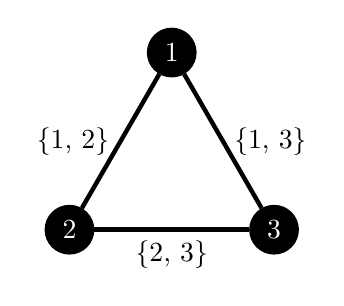
\begin{tikzpicture}[
    main node/.style={circle,fill=black,draw,text=white},
    edge label/.style={midway, auto}
]
    \def\R{1.5}
    \node[main node] (1) at (90:\R) {1};
    \node[main node] (2) at (210:\R) {2};
    \node[main node] (3) at (330:\R) {3};

  \draw[ultra thick] (1) -- (2) node[edge label, left] {\{1, 2\}};
  \draw[ultra thick] (2) -- (3) node[edge label, below] {\{2, 3\}};
  \draw[ultra thick] (1) -- (3) node[edge label, right] {\{1, 3\}};
\end{tikzpicture}
\caption{例1における無向ネットワーク $(N, G)$}
\label{fig:2.1}
\end{figure}
\end{example}
\vspace{0.5cm}

ネットワーク形成関数 $G: \prod_{i \in N} \{0,1\}^{n-1} \rightarrow \mathcal{G}$ は, $G(\bm{g}) := \{\{i,j\} \in \binom{N}{2}\ |\ g_{i,j} = g_{j,i} = 1\}$ に従い, リンク表明ベクトル $\bm{g}$ を無向ネットワークへと写像する. 
結果として得られるネットワークを $(N, G(\bm{g}))$ と書く. 
リンク表明ベクトル $\bm{g}$ が文脈上明らかである場合は $G(\bm{g})$ の代わりに単に $G$ と書き, 同様にエージェント集合が自明な場合は $(N, G)$ の代わりに単に $G$ と表記する. 
$G$ における $i$ の近傍を $N_i(G) = \{j \in N \setminus \{i\} : \{i,j\} \in G\}$ とし, $i$ の次数を $d_i(G) = |N_i(G)|$ と定義する. 
自己ループは存在しないため, 自身が近傍に含まれることはない. 
また, $N_i(G) = \emptyset$ の場合, エージェント $i$ は孤立している (Isolated) と呼ぶ.

ネットワーク $G$ が与えられたとき, $G + \{i,j\}$ と $G - \{i,j\}$ は以下のように解釈される. 
$G + \{i,j\}$ は, リンク $\{i, j\}$ をネットワーク $G$ に追加することを意味し, 厳密には $G' = G + \{i,j\}$, もしくは和集合を用いて $G' = G \cup \{\{i,j\}\}$ と記される. 
$G - \{i,j\}$ は, リンク $\{i, j\}$ をネットワーク $G$ から削除することを意味し, 厳密には $G' = G - \{i,j\}$, もしくは差集合を用いて $G' = G \setminus \{\{i,j\}\}$ と記される.

\vspace{0.5cm}
\begin{example}
$N = \{1, 2, 3\},\ \bm{g_1'}=(0, 1),\ \bm{g_2'}=(1, 1),\ \bm{g_3'}=(1, 0)$ とする. 
このとき, $G'(\bm{g})=\{\{1, 3\}\}$となる. 
これは, 例1の場合と比較すると, リンク表明ベクトルは $\bm{g_1'}=\bm{g_1}-\{1, 2\},\ \bm{g_3'}=\bm{g_3}-\{1, 3\}$ である. 
そのため, $\bm{g_1'}\subseteq \bm{g_1},\ \bm{g_3'}\subseteq \bm{g_3}$となる. 
また, ネットワーク形成関数は $G'=G-\{1, 2\}-\{2, 3\}$ となる. 
したがって, 無向ネットワーク$(N, G')$ は図\ref{fig:2.2}のような形となる.

また, それぞれのエージェントの近傍は $N_1(G')=\{3\},\ N_2(G')=\{\emptyset\},\ N_3(G')=\{1\}$ であり, 次数は $d_1(G')=|N_1(G')|=1,\ d_2(G')=|N_2(G')|=0,\ d_3(G')=|N_3(G')|=1$ である. 
このとき, $N_2(G')=\emptyset$ であるため, エージェント2は孤立しているという.

\begin{figure}[htbp]
\centering
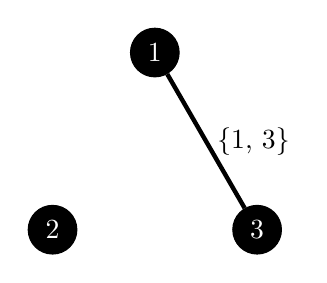
\begin{tikzpicture}[
    main node/.style={circle,fill=black,draw,text=white},
    edge label/.style={midway, auto}
]
    \def\R{1.5}
    \node[main node] (1) at (90:\R) {1};
    \node[main node] (2) at (210:\R) {2};
    \node[main node] (3) at (330:\R) {3};
    
    \draw[ultra thick] (1) -- (3) node[edge label, right] {\{1, 3\}};
\end{tikzpicture}
\caption{例2における無向ネットワーク $(N, G')$}
\label{fig:2.2}
\end{figure}
\end{example}
\vspace{0.5cm}

次に, 本論文における利得関数を定義する. 

戦略プロファイル $\bm{s}$ の下でのエージェント $i$ の利得は次式で与えられる.
\[
\Pi_i(\bm{s}(\bm{x}, \bm{g})) = \pi_i(x, G(\bm{g})) - d_i(G(\bm{g}))\kappa,
\]
ここで $\kappa > 0$ はリンク費用を表す. 
また, リンク費用を除く利得(粗利得)関数 $\pi_i(\bm{x}, G(\bm{g}))$ は, Ballester et al. (2006) によって提案された, ローカルな戦略的補完性とグローバルな戦略的代替性を併せ持つ以下の線形二次利得関数によって定義される.
\[
\pi_i(\bm{x},G(\bm{g})) = \alpha x_i - \frac{1}{2}(\beta+\gamma)x_i^2 + \lambda x_i \sum_{j \in N_i(G)}x_j - \gamma x_i \sum_{j \in N \setminus \{i\}}x_j \quad \text{for all } i \in N
\]
ただし, $\alpha > 0, \beta > 0, \lambda > 0, \gamma \ge 0$ である.

上記の総利得関数 $\pi_i(\bm{x}, G(\bm{g}))$ の各パラメータの経済学的含意は以下の通りである. 
$\alpha$ は, エージェントが努力を発揮することから得られる自律的利得 (Stand-alone Benefit) を表す. 
この利得は他のエージェントの行動には依存しない. 
項 $(\beta+\gamma)$ は, 努力を発揮するために必要となる費用を表すパラメータである. 
$\lambda$ は, ローカルな正の外部性と戦略的補完性の強さを表す. 
すなわち, 近傍の努力水準が自身の利得をどれだけ高めるか, および近傍の総努力水準の増加に対して自身の努力水準を引き上げるインセンティブの大きさを決定する. 
最後に $\gamma$ は, グローバルな負の外部性と戦略的代替性の強さを表す. 
すなわち, ネットワーク上の他のすべてのエージェントの総努力水準によって被る負の影響の大きさ, および他者の総努力水準の増加に対して自身の努力水準を引き下げるインセンティブの大きさを決定する.

本論文では, 分析対象となる応用例に従い $\lambda \ge \gamma$ を仮定する. 
これにより, 直接つながっているエージェント間では努力水準が戦略的補完関係(正の外部性)にあることが保証される. 
また, 任意の固定ネットワーク $G$ に対して努力水準のナッシュ均衡の存在と一意性を保証するために, Ballester et al. (2006) に則り, $\beta > (n-1)\lambda$ を仮定する.

$G$ におけるエージェント $i$ の近傍の総努力水準\footnote{$i$ のアクセス努力水準 (Accessed Effort Level) とも呼ぶ.}を $y_i(x_{-i}, G) := \sum_{j \in N_i(G)}x_j$ と表記し, $i$ 以外のすべてのエージェントの総努力水準を $z_i(x_{-i}, G) := \sum_{j \in N \setminus \{i\}}x_j$ と表記する. 
$x_{-i}$ が文脈上明らかな場合は, 簡略化のために $y_i(G)$ および $z_i(G)$ と記述する. 
$\pi_i(\bm{x}, G(\bm{g}))$ を $x_i$ に関して最大化することで\footnote{具体的には, $\pi_i(\bm{x}, G(\bm{g}))$ を $x_i$ で偏微分し, 一階条件を解くことで得られる.}, 以下の最適反応努力水準 $\overline{x}_i(y_i(G), z_i(G))$ が得られる.
\[
\overline{x}_i(y_i(G), z_i(G)) \equiv \overline{x}_i(x_{-i}, G) = \frac{1}{\beta+\gamma} \left( \alpha + \lambda \sum_{j \in N_i(G)}x_j - \gamma \sum_{j \in N \setminus \{i\}}x_j \right).
\]
この $\overline{x}_i(y_i(G), z_i(G))$ を $\pi_i(\overline{x}_i, x_{-i}, G)$ に代入することで, 以下の価値関数 $v_i(y_i(G), z_i(G))$ が得られる.
\[
v_i(y_i(G), z_i(G)) \equiv \pi_i(\overline{x}_i, x_{-i}, G) = \frac{1}{2(\beta+\gamma)} \left( \alpha + \lambda \sum_{j \in N_i(G)}x_j - \gamma \sum_{j \in N \setminus \{i\}}x_j \right)^2.
\]

\subsubsection*{ペアワイズナッシュ均衡}
本論文で採用する安定性概念は, 通常のナッシュ均衡を精緻化させたペアワイズナッシュ均衡である. 
この概念は, エージェントがペアで逸脱し, 新たなリンクを形成しつつ, 互いの努力水準を最適反応へと調整する状況を考慮に入れる. 
具体的には, エージェント $i$ と $j$ が新しいリンク $\{i, j\}$ を形成するために逸脱する場合, 逸脱時の努力水準 $\overline{x}_i'(G+\{i,j\})$ と $\overline{x}_j'(G+\{i,j\})$ は相互に最適反応であると仮定される.

\vspace{0.5cm}
\begin{definition}[\textbf{ペアワイズナッシュ均衡}]
戦略プロファイル $\bm{s}=(\bm{x}, \bm{g})$ は, 以下の2つの条件を満たすとき, ペアワイズナッシュ均衡である.
\begin{enumerate}
    \item \textbf{ナッシュ均衡条件:}
    すべてのエージェント $i\in N$ およびすべての戦略 $\bm{s_{i}}\in S_{i}$ について, 以下が成立する.
    \[
    \Pi_{i}(\bm{s})\ge\Pi_{i}(\bm{s_{i}}, \bm{s_{-i}})
    \]
    すなわち, どのエージェントも単独で努力水準やリンク表明の戦略を変更して利得を高めることはできない.

    \item \textbf{ペアワイズ安定性:}
    現在のネットワーク $G(\bm{g})$ に存在しないすべてのリンク $\{i,j\} \notin G(\bm{g})$ について, $\overline{x}_i'(G+\{i,j\})$ と $\overline{x}_j'(G+\{i,j\})$ を以下の解として定義する.
    \begin{align*}
        \overline{x}_i'(G+\{i,j\}) &= \overline{x}_i(y_i(G) + \overline{x}_j'(G+\{i,j\}), z_i(G) + \overline{x}_j'(G+\{i,j\}) - x_j), \\
        \overline{x}_j'(G+\{i,j\}) &= \overline{x}_j(y_j(G) + \overline{x}_i'(G+\{i,j\}), z_j(G) + \overline{x}_i'(G+\{i,j\}) - x_i).
    \end{align*}
    エージェント $i$ と $j$ がリンク $\{i, j\}$ を形成し, それに応じて努力を調整する一方で, 他のすべての努力が固定されたままであるという逸脱の下でのエージェント $i$ への利得を以下のように定義する.
    \[
    \Pi_i'(G+\{i,j\}) := \Pi_i(\overline{x}_i'(G+\{i,j\}), \overline{x}_j'(G+\{i,j\}), x_{-i,-j}, G+\{i,j\})
    \]
    エージェント $j$ への利得 $\Pi_j'(G+\{i,j\})$ も同様に定義する.

    もし, 
    \[
    \Pi_i'(G+\{i,j\}) > \Pi_i(\bm{s})
    \]
    ならば, 
    \[
    \Pi_j'(G+\{i,j\}) < \Pi_j(\bm{s}).
    \]
    が成立する. 
\end{enumerate}
\end{definition}

この定義は, ペアワイズナッシュ均衡がリンクの追加に対して頑健であることを示している. 
つまり, 新たにリンクを形成することで, 両方のエージェントが厳密に利得を改善すること, あるいは一方が厳密に改善しもう一方が現状維持となるような状況は存在しない.

なお, ペアワイズナッシュ均衡は, エージェントのペアがリンクを形成すると同時に既存のリンクを削除するような逸脱は考慮していない点に留意が必要である. 
また, 本設定におけるペアワイズナッシュ均衡ネットワークは, 必ず入れ子分割グラフ (Nested Split Graph) の構造を持つことが知られている.

本論文では構成 (Configuration) という用語を使用し, ネットワーク $G$ と対応するナッシュ均衡努力水準のベクトル $\bm{x}(G)$ を $(\bm{x}(G), G)$ と表記する. 
構成 $(\bm{x}(G), G)$ においてエージェント $i$ がエージェント $j$ とのリンクを形成するとき, エージェント $i$ の限界粗利得を $\Delta v_i(G+\{i,j\})$ と書く. 
同様に, 構成 $(\bm{x}(G), G)$ において, エージェント $i$ がエージェント集合 $W$ に含まれるエージェントとのリンクを削除(あるいは維持を撤回)する場合の限界粗利得を $\Delta v_{i}(G-\sum_{j\in W}\{i,j\})$ と表記する.

また, 数式をパラメータ $\gamma$ の関数として記述し, 引数の一つとして $\gamma$ を明示的に加えることがある. 
例えば, ナッシュ均衡努力水準ベクトルを $\bm{x}(G,\gamma)$ と表記する. 
本論文を通じて, ある結果が「$\gamma$ が十分に小さい場合に成立する」と言うときは, ある $\overline{\gamma}>0$ が存在し, すべての $\gamma\in[0,\overline{\gamma}]$ においてその結果が成立することを意味するものとする.

\subsubsection*{グラフ理論の概念と表記}
本分析において重要となるグラフ理論の諸概念および表記について定義する. 
ここでは, ネットワーク間の構造的な比較, エージェント排除後のネットワークの定義, そして均衡ネットワークが満たす特定のグラフの形について述べる.

まず, 2つのネットワーク $(N, G)$ と $(N', G')$ の関係性を次のように定義する.

\vspace{0.5cm}
\begin{definition}[\textbf{同型 (Isomorphism)}]
ある全単射写像 $f:N\rightarrow N'$ が存在し, 任意の $\{i,j\}$ について, $\{i,j\}\in G$ であることと $\{f(i),f(j)\}\in G'$ であることが同値となるとき, ネットワーク $(N, G)$ と $(N', G')$ は同型であるという. 
これは, エージェントのラベルを付け替えることで2つのネットワークが完全に一致することを意味する. 
便宜上, $(N, G)$ と $(N', G')$ が同型である場合, 単に $G=G'$ と表記する.
\end{definition}

\begin{definition}[\textbf{被覆 (Covering)}]
ある全単射写像 $f:N\rightarrow N'$ が存在し, リンク集合に関して $\{\{i,j\}:\{i,j\}\in G\}\subset\{\{f(i),f(j)\}:\{f(i),f(j)\}\in G'\}$ が成立するとき, ネットワーク $(N', G')$ は $(N, G)$ を被覆するという. 
本論文では, $(N', G')$ が $(N, G)$ を被覆する関係を $G\subset G'$ と表記する. 
また, 2つのネットワークが同型であるか, または被覆関係にある場合を総称して $G\subseteq G'$ と記す.
\end{definition}
\vspace{0.5cm}

政策的介入によってネットワークから一部のエージェントが取り除かれる状況を以下のように定式化する. 
ネットワーク $(N,G)$ からエージェントの部分集合 $E\subset N$ が排除されたとする. 
このとき, 残存するネットワークを $(N\setminus E, G(E))$ と表記する. 
ここで $G(E)$ は, $E$ に属さないエージェント間のリンクのみを残したリンク集合である. 
すなわち, $(N\setminus E, G(E))$が$\{i,j\}\in G(E)$ であるための必要十分条件は, $i,j\in N\setminus E$ かつ $\{i,j\}\in G$ である.

続いて, 本論文の分析において中心的な役割を果たすグラフ構造として, 入れ子分割グラフを定義する.

\vspace{0.5cm}
\begin{definition}[\textbf{入れ子分割グラフ (Nested Split Graph)}]
ネットワーク $G$ において, あるエージェント $i$ の次数が $j$ の次数以上である ($d_{i}(G)\ge d_{j}(G)$) とき, $j$ の近傍が必ず $i$ の近傍に含まれるならば, そのときの $G$ を入れ子分割グラフと呼ぶ.
形式的には, 以下の条件が満たされる場合である.
\[
\{j,k\}\in G \quad \text{かつ} \quad d_{i}(G)\ge d_{j}(G) \implies \{i,k\}\in G
\]
この構造では, 次数の高いハブ的なエージェントは, 次数の低いエージェントがつながっている相手とは必ずつながっているという階層性を持つ.
\end{definition}

\vspace{0.5cm}
\begin{example}
    入れ子分割グラフの例を図\ref{fig:2.3}に示す. 
    このグラフでは, エージェント1が次数4のハブ的エージェントであり, 他のすべてのエージェントとつながっている. 
    エージェント2は次数2であり, エージェント1およびエージェント3とつながっている. 
    これにより, $N(4)=\{1\} ⊂ N(2)=\{1,3\} ⊂ N(1)=\{2,3,4,5\}$ のような包含関係が成立していることがわかる.

\begin{figure}[htbp]
\centering
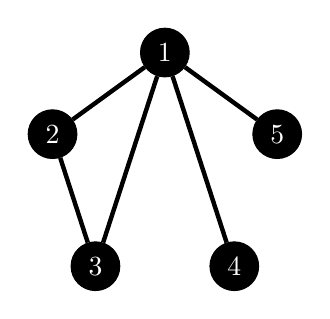
\begin{tikzpicture}[
    main node/.style={circle,fill=black,draw,text=white},
    ]
  \def\R{1.5}

  \node[main node] (1) at (90:\R) {1};
  \node[main node] (2) at (162:\R) {2};
  \node[main node] (3) at (234:\R) {3};
  \node[main node] (4) at (306:\R) {4};
  \node[main node] (5) at (18:\R) {5};

  \draw[ultra thick] (1) -- (2);
  \draw[ultra thick] (1) -- (3);
  \draw[ultra thick] (1) -- (4);
  \draw[ultra thick] (1) -- (5);

  \draw[ultra thick] (2) -- (3);
\end{tikzpicture}
\caption{入れ子分割グラフ (Nested Split Graph) の例}
\label{fig:2.3}
\end{figure}
\end{example}
\vspace{0.5cm}

また, 特殊なケースとして, すべての $i, j \in N$ について $\{i,j\} \notin G$ であるネットワーク\footnote{すなわち, どのエージェント間にもリンクが存在しないネットワーク.}を空ネットワーク (Empty Network) と呼び, $G^e$ と表記する. 
$i \ne j$ であるすべての $i, j \in N$ について $\{i,j\} \in G$ であるネットワーク\footnote{すなわち, 異なるすべてのエージェント間にリンクが存在するネットワーク.}を完全ネットワーク (Complete Network) と呼び, $G^c$ と表記する.

\vspace{0.5cm}
\begin{example}
    $N=\{1,2,3,4,5\}$ のときの空ネットワーク $G^e$ と完全ネットワーク $G^c$ は, 図\ref{fig:2.4}および図\ref{fig:2.5}のようになる.
    
    \begin{figure}[htbp]
    \begin{tabular}{c|c}
    \begin{minipage}{0.45\linewidth}
    \centering
    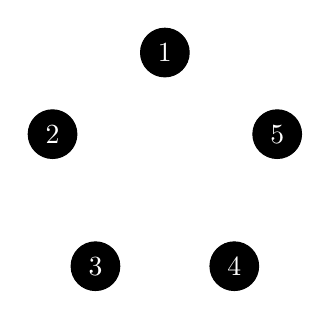
\begin{tikzpicture}[
        main node/.style={circle,fill=black,draw,text=white},
    ]
    
    \def\R{1.5}
    \node[main node] (1) at (90:\R) {1};
    \node[main node] (2) at (162:\R) {2};
    \node[main node] (3) at (234:\R) {3};
    \node[main node] (4) at (306:\R) {4};
    \node[main node] (5) at (18:\R) {5};
    \end{tikzpicture}
    \caption{例4における空ネットワーク $G^e$}
    \label{fig:2.4}
    \end{minipage} &

    \begin{minipage}{0.45\linewidth}
    \centering
    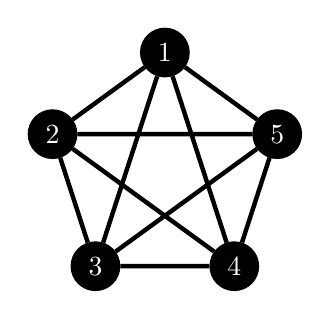
\begin{tikzpicture}[
        main node/.style={circle,fill=black,draw,text=white},
        ]
    
    \def\R{1.5}
    
    \node[main node] (1) at (90:\R) {1};
    \node[main node] (2) at (162:\R) {2};
    \node[main node] (3) at (234:\R) {3};
    \node[main node] (4) at (306:\R) {4};
    \node[main node] (5) at (18:\R) {5};
    
    \draw[ultra thick] (1) -- (2) -- (3) -- (4) -- (5) -- (1) -- (3) -- (5) -- (2) -- (4) -- (1);
    \end{tikzpicture}
    \caption{例4における完全ネットワーク$G^c$}
    \label{fig:2.5}
    \end{minipage}
    \end{tabular}
    \end{figure}
\end{example}
\vspace{0.5cm}

\subsection{ペアワイズ最適反応ダイナミクスと最適ターゲティング政策}
本節では, まず計画者による介入後のエージェントの調整行動を記述する動学モデルを導入し, 次にそのモデルに基づいた最適ターゲティング政策を定義する.

\subsubsection{ペアワイズ最適反応ダイナミクス}
計画者がネットワーク $G$ からエージェント集合 $E$ を排除した後, 残存するエージェントがリンクおよび努力水準を調整行動をペアワイズ最適反応ダイナミクスとしてモデル化する. 
これは時系列 $t=0, 1, 2, \dots$ における無限期間の調整過程である. 
計画者はエージェントの調整行動を考慮に入れた上で, 最大 $e$ 人のエージェントを排除することで, 各期の総努力水準を現在価値で割り引いた割引総努力水準 (Discounted Aggregate Effort Levels) を最小化することを目指す. 
リンク形成とリンク削除は異なるタイミングで行われると仮定する. 
具体的には以下の手順で進行する.

\begin{itemize}
    \item \textbf{$t=0$:エージェントの排除}
    
    計画者がネットワーク $G$ からエージェント集合 $E \subseteq N$ を排除する. 
    これにより, $E$ に属するすべてのエージェントおよび $E$ 内のエージェントと接続しているすべてのリンクが排除される. 
    そのため, 第0期の結果として得られるネットワークは, $(N \setminus E, G_0(E))$ で与えられる. 
    したがって, 第0期におけるネットワーク $G_{0}(E)$ は以下のように定義される.
    \[
    G_{0}(E) := \{\{i,j\} \in G : i, j \notin E\}
    \]
    このとき, ネットワークの構成は $(\bm{x}(G_{0}(E)), G_{0}(E))$ となる.

    \vspace{0.5cm}
    \begin{example}
        $(N, G)$ が $N=\{1, 2, 3, 4\}$, $G=\{\{1, 2\}, \{1, 3\}, \{1, 4\}, \{2, 3\}, \{2, 4\}\}$ であり, $E=\{2,3\}$ であると仮定する. このとき, $(N \setminus E, G_0(E))$ は $N \setminus E = \{1,4\}$ かつ $G_0(E) = \{\{1,4\}\}$ となる. 図\ref{fig:2.6}および図\ref{fig:2.7}に, 排除前および排除後のネットワークを示す. 特に, 図\ref{fig:2.6}において赤色で示されたエージェントとリンクが排除されることに注意されたい.

            \begin{figure}[htbp]
            \begin{tabular}{c|c}
            \begin{minipage}{0.45\linewidth}
            \centering
            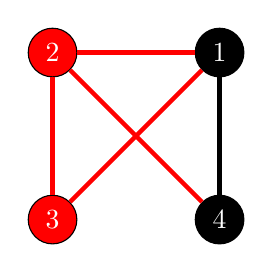
\begin{tikzpicture}[
                main node/.style={circle,fill=black,draw,text=white},
                ]
                \def\R{1.5}
                \node[main node] (1) at (45:\R) {1};
                \node[main node, fill=red] (2) at (135:\R) {2};
                \node[main node, fill=red] (3) at (225:\R) {3};
                \node[main node] (4) at (315:\R) {4};
                
                \draw[ultra thick, red] (1) -- (2);
                \draw[ultra thick, red] (1) -- (3);
                \draw[ultra thick] (1) -- (4);
                \draw[ultra thick, red] (2) -- (3);
                \draw[ultra thick, red] (2) -- (4);
            \end{tikzpicture}
            \caption{例5における排除前のネットワーク $(N, G)$}
            \label{fig:2.6}
            \end{minipage} &
            
            \begin{minipage}{0.45\linewidth}
            \centering
            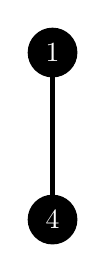
\begin{tikzpicture}[
                main node/.style={circle,fill=black,draw,text=white},
                ]
                \def\R{1.5}
                \node[main node] (1) at (45:\R) {1};
                \node[main node] (4) at (315:\R) {4};

                \draw[ultra thick] (1) -- (4);
            \end{tikzpicture}
            \caption{例5における排除後のネットワーク $(N \setminus E, G_0(E))$}
            \label{fig:2.7}
        \end{minipage}
        \end{tabular}
        \end{figure}
    \end{example}
    \vspace{0.5cm}

    \item \textbf{$t$ が奇数:リンク形成}
    
    任意の奇数期 $t$ において, 構成 $(\bm{x}(G_{t-1}(E)), G_{t-1}(E))$ を所与として, 次の条件を満たす, 有益となるすべての新たなリンクを形成する. 
    リンク $\{i,j\} \notin G_{t-1}(E)$ について, 以下の条件が満たされる場合, そのリンクは $G_{t}(E)$ に追加される.
    \[
    \Pi_{i}'(G+\{i,j\}) \ge \Pi_{i}(\bm{s}) \quad \text{かつ} \quad \Pi_{j}'(G+\{i,j\}) \ge \Pi_{j}(\bm{s})
    \]
    ただし, 少なくとも一方の不等号は厳密に成立する必要がある. 
    これによって, ネットワーク $G_t(E)$が得られる.

    \item \textbf{$t$ が偶数:リンク削除}
    
    $t\ge2$ の任意の偶数期 $t$ において, エージェントは既存のリンクを一方的に削除する機会を持つ. 
    リンクの形成には双方の合意が必要であるが, リンクの維持(または削除)は各エージェントの単独の意思決定によって行われる点が重要である. 
    本モデルでは分析の便宜上, 構成 $(\bm{x}(G_{t-1}(E)), G_{t-1}(E))$ が与えられたとき, エージェントは極大リンク削除最適反応 (Maximal Link Deletion Best Response) に従うと仮定する. 
    これによりネットワーク $G_t(E)$ が得られる.
    
    まず, 通常のリンク削除最適反応 (Link Deletion Best Response) を定義するために, いくつかの表記を導入する. 
    先述した通り, $\bm{g}$ はすべてのエージェントのリンク表明のベクトル, すなわち $\bm{g} = (g_1, g_2, ..., g_n)$ を表すため, $\bm{g}$ を $(\bm{g_i}, \bm{g_{-i}})$ と書くことができる. 
    ここで $\bm{g_{-i}}$ はエージェント $i$ を除くすべてのエージェントのリンク表明を表す. 
    
    エージェント $i$ が $\bm{g_i'}$ に逸脱し, $(\bm{g_i'}, \bm{g_{-i}})$ という結果になると仮定する. 
    表記を乱用して, $(\bm{g_i'}, \bm{g_{-i}})$ によって導出される無向ネットワークを $G_i'$ と書く. 
    つまり, $G_i' := G(\bm{g_i'}, \bm{g_{-i}})$ として得られる. 
    エージェント $i$ が現在のリンク表明 $\bm{g_{i}}$ の部分集合 $\bm{g_{i}'} \subseteq \bm{g_{i}}$ へと逸脱した際の逸脱利得を $\Pi_{i}'(G_{i}')$ とする. 
    
    この逸脱の下でのエージェント $i$ の最適反応努力水準は $\overline{x}_i'(x_{-i}(G), G_i')$ で与えられ\footnote{このとき, 他のすべてのエージェントの努力は固定されたままである.}, 逸脱利得を以下のように定義する.
    \[
    \Pi_i'(G_i') := \Pi_i(\overline{x}_i'(x_{-i}(G), G_i'), x_{-i}(G), G_i').
    \]
    これは, 現在の構成 $(\bm{x}(G), G)$ と比較した, リンクを切断し努力水準をそれに応じて調整することによるエージェント $i$ の効用を表す.

    \vspace{0.5cm}
    \begin{definition}[\textbf{リンク削除最適反応 (Link Deletion Best Response)}]
        構成 $(\bm{x}(G), G)$ を考える. 
        リンク削除最適反応 $\bm{g_i'} \subseteq \bm{g_i}$ とは, $\bm{g_i'} \in \arg \max_{\bm{g}: \bm{g} \subseteq \bm{g_i}} \Pi_i'(G_i')$ となるエージェント $i$ のリンク表明ベクトルである. 
        リンク削除最適反応 $\bm{g_i'}$ は, 現在のネットワーク $G$ と $\bm{x}(G)$ における残りのエージェントの努力水準が与えられたとき, エージェント $i$ の逸脱利得を最大化するエージェント $i$ の現在のリンク表明ベクトル $\bm{g_i}$ の部分集合である.
    \end{definition}
    \vspace{0.5cm}
    
    次に, 極大リンク削除最適反応を定義する. 
    極大リンク削除最適反応は, リンク削除最適反応が存在する場合, エージェントは可能な限り多くのリンクを削除するものとして定義される.
    
    \vspace{0.5cm}
    \begin{definition}[\textbf{極大リンク削除最適反応 (Maximal Link Deletion Best Response)}]
        構成 $(\bm{x}(G), G)$ を考える. 
        極大リンク削除最適反応 $\bm{g_i^m} \subseteq \bm{g_i}$ とは, 以下の条件を満たすエージェント $i$ のリンク表明ベクトルである.
        \begin{itemize}
            \item もし, $\bm{g_i} \in \arg \max_{\bm{g}: \bm{g} \subseteq \bm{g_i}} \Pi_i'(G_i')$ ならば, $\bm{g_i^m} = \bm{g_i}$.
            \item もし, $\bm{g_i} \notin \arg \max_{\bm{g_i'}: \bm{g_i'} \subseteq \bm{g_i}} \Pi_i'(G_i')$ ならば, 以下の2つの条件を満たす.
            \begin{itemize}
                \item $\bm{g_i^m} \in \arg \max_{\bm{g_i'}: \bm{g_i'} \subseteq \bm{g_i}} \Pi_i'(G_i')$ である.
                \item 他の任意の $\bm{g_i'} \in \arg \max_{\bm{g_i'}: \bm{g_i'} \subseteq \bm{g_i}} \Pi_i'(G_i')$ に対して, $\bm{g_i^m} \subseteq \bm{g_i'}$ が成立する.
            \end{itemize}
        \end{itemize}
    \end{definition}
    \vspace{0.5cm}
\end{itemize}

極大リンク削除最適反応の定義は, リンク削除最適反応の概念を精緻化したものであり, 2つの場合に分けられる. 
第一に, 構成 $(\bm{x}(G), G)$ におけるエージェント $i$ の現在のリンク表明 $\bm{g_i}$ がリンク削除最適反応である場合, 極大リンク削除最適反応は単に $\bm{g_i}$ であると述べている. 
第二に, $\bm{g_i}$ がリンク削除最適反応でない場合, 極大リンク削除最適反応は, リンク表明が最小かつリンク削除が最大となるようなリンク削除最適反応として定義される. 
Hiller (2025) の補題7より, 最適反応関数が適切に定義されており, エージェント数が有限であると仮定しているため, 極大リンク削除最適反応は常に存在する. 
さらに, 価値関数の凸性により, 極大リンク削除最適反応は常に一意に定まる.

\subsubsection{最適ターゲティング}

最適ターゲティング政策 (Optimal Targeting Policy)とは, ペアワイズナッシュ均衡にあるネットワーク $G$ から排除することで割引総努力水準を最小化するエージェントの集合を特定する. 
割引因子を $\delta \in (0,1)$ と表記する. 

計画者がネットワークから排除可能なエージェントの最大数を $e$ ($1 \le e < n$) とする. 
計画者は $e$ 人未満のエージェントを排除することも可能であり, 介入を行わないという選択肢も含まれる.

\vspace{0.5cm}
\begin{definition}[\textbf{最適ターゲティング政策 (Optimal Targeting Policy)}]
    エージェント集合 $E \subset N$ は, 以下の計画者問題の解であるとき, 最適ターゲティング政策と呼ばれる.
\[
\min_{E \subset N} \sum_{t=0}^{\infty} \delta^t \sum_{j \in N \setminus E} x_j(G_t(E))\qquad \text{subject to } |E| \le e.
\]
\end{definition}
\vspace{0.5cm}

ここで, $G_{t}(E)$ はエージェント集合 $E$ を排除した後に, 前節で定義されたペアワイズ最適反応ダイナミクスに従って $t$ 期に形成されるネットワークを表す. 
$x_{j}(G_{t}(E))$ はそのネットワークにおけるエージェント $j$ のナッシュ均衡努力水準である.

この定義は, 計画者が単に介入直後の静的な結果だけでなく, ネットワークの形状と努力水準が将来にわたって適応していく動的な過程全体を評価し, 最適化を行うことを示している.

\section{分析}
本章では, グローバルな戦略的代替効果を表すパラメータ $\gamma$ の大きさに応じて, 最適ターゲティング政策がどのように変化するかを分析する.

第1節では $\gamma$ が小さい場合の最適ターゲティング政策を提示し, 第2節では $\gamma$ が大きい場合について提示する.

\subsection{$\gamma$ が十分に小さい場合の最適ターゲティング}
本節では, グローバルな戦略的代替効果を統御するパラメータ $\gamma$ が十分に小さい場合における最適ターゲティング政策について分析する. 
この場合, ネットワークの適応過程は比較的単純化され, 直感的な次数に基づく政策が最適となることが示される. 
分析に先立ち, まず本節の主要結果を記述するために必要となる次数極大集合 (Degree-Maximal Set) の概念を定義する.

\subsubsection{次数極大集合}
最適ターゲティング政策を特徴付けるために, ネットワーク内で最も次数の高いエージェントの集合を形式的に定義する. 
これを定義8として以下に示す.

\vspace{0.5cm}
\begin{definition}[\textbf{次数極大集合 (Degree-Maximal Set)}]
ネットワーク $(N, G)$ において, 以下の概念を定義する.

\begin{itemize}
    \item \textbf{次数極大集合 (Degree-Maximal Set):}
    エージェントの部分集合 $A \subset N$ が次数極大であるとは, $A$ に属するすべてのエージェント $i$ の次数が, $A$ に属さない任意のエージェント $j$ の次数以上である状態を指す.
    \[
    d_{i}(G) \ge d_{j}(G) \quad \forall i \in A, \forall j \in N \setminus A
    \]
    
    \item \textbf{次数極大集合族 (Family of Degree-Maximal Sets) :}
    濃度が $a$ であるような次数極大集合の族を $\mathcal{E}(a)$ と表記する.
    \[
    \mathcal{E}(a) = \{ A \subset N : |A|=a \text{ かつ } d_{i}(G) \ge d_{j}(G) \quad \forall i \in A, \forall j \in N \setminus A\}\notag
    \]
\end{itemize}
\end{definition}
\vspace{0.5cm}
したがって, 部分集合 $A \subset N$ は, $A$ 内のすべてのエージェント $i$ が $A$ に属さない任意のエージェント $j$ 以上の次数を持つ場合, 次数最大と呼ばれる. 
集合の族 $\mathcal{E}(a)$ は, 濃度 $a$ のすべての次数最大集合からなる. 
より形式的には, 集合 $A$ がちょうど $a$ 人のエージェントを持ち, $A$ 内のすべてのエージェントが $A$ に属さない任意のエージェントの次数以上である場合, $A$ は $\mathcal{E}(a)$ に属する.

\subsubsection{最適ターゲティング政策:次数に基づくカットオフルール}
$\gamma$ が十分に小さい場合, 最適ターゲティング政策は, 上記で定義した次数極大集合を排除することと同等である.
ただし, 排除可能なエージェントの最大数 $e$ は, 計画者が第0期に空ネットワークを取得できないような数であると仮定することに注意されたい. 
これは, 閾値を $t(G)$ とした場合に, 条件 $e < t(G)$ によって保証される.

閾値 $t(G)$ は, 次のように導出される. 
\begin{equation}
    t(G) :=\notag
    \begin{cases}
    |\mathcal{D}_{rel}(G)| \quad & k \text{が奇数のとき}, \\
    |\mathcal{D}_{rel}(G)| - 1 \quad & k \text{が偶数のとき}.
    \end{cases}
\end{equation}
ここで, $\mathcal{D}_{rel}(G)$ を定義するために, Hiller (2025) のOnline Appendixに収録されている補題OA1, 及び定義OA5を用いる.

本補題においては, ネットワーク $(N, G)$ を考え, $\mathcal{D}(G) = (\mathcal{D}_0(G), \mathcal{D}_1(G), ..., \mathcal{D}_k(G))$ をその次数分割 (Degree Partition) とする. 
このとき, 以下は同値であることが知られている.

\begin{itemize}
    \item ネットワーク $G$ は入れ子分割グラフである.
    \item エージェントの集合 $N$ は, 独立集合 $D_j(G), (j = 1, ..., \lfloor k/2 \rfloor)$ と相対的支配集合 (Relative Dominating Set) $\bigcup_{j=\lfloor k/2\rfloor+1}^{k} \mathcal{D}_j(G)$ に分割できる. 
    さらに, 近傍は入れ子となっており, 具体的には, 各エージェント $i \in D_j(G), j=1, ..., k$ に対して, 次の条件式が成立する.
    \begin{equation}
    N_i(G) :=\notag
    \begin{cases}
    \bigcup_{l=1}^{j} \mathcal{D}_{k+1-l}(G) \quad & j=1, ..., \lfloor k/2\rfloor \text{のとき}, \\
    \bigcup_{l=1}^{j} \mathcal{D}_{k+1-l}(G) \setminus \{i\} \quad & j=\lfloor k/2\rfloor+1, ..., k \text{のとき}.
    \end{cases}
\end{equation}
\end{itemize}

\vspace{0.5cm}
\noindent\textbf{定義OA5 (結合独立集合と相対的支配集合).}
    ネットワーク $(N, G)$ を考え, その次数分割を $\mathcal{D}(G) = (\mathcal{D}_0(G), \mathcal{D}_1(G), ..., \mathcal{D}_k(G))$ とするとき, 結合独立集合 (Combined Independent Set) $\mathcal{I}(G)$ と相対的支配集合 (Relative Dominating Set) $\mathcal{D}_{rel}(G)$ をそれぞれ以下のように定義する.
    \begin{itemize}
        \item 結合独立集合は,  $\mathcal{I}(G) = \bigcup_{j=1}^{\lfloor k/2\rfloor} \mathcal{D}_{j}(G)$ の和集合として定義される.
        \item 相対的支配集合は,  $\mathcal{D}_{rel}(G) = \bigcup_{j=\lfloor k/2\rfloor + 1}^{k} \mathcal{D}_{j}(G)$ の和集合として定義される.
    \end{itemize}
\vspace{0.5cm}

Hiller (2025) の補題OA1から, 結合独立集合 $\mathcal{I}(G)$ 自体が入れ子分割グラフ $(N, G)$ の独立集合であることは, 直接的にわかる.
さらに, $(N, G)$ が $\mathcal{D}_0(G)$ が空であるような入れ子分割グラフであれば, 相対的支配集合 $\mathcal{D}_{rel}(G)$ は $(N, G)$ の支配集合である. 
最後に, $G$ が空のネットワークである場合, ネットワーク $G(\mathcal{D}_0)$ においてエージェントの集合 $N \setminus \mathcal{D}_0$ は空であることに注意されたい. 
したがって, 集合 $\mathcal{D}_{rel}$ は空である.

以上より, 閾値 $t(G)$ は計画者が排除可能なエージェントの最大数が $t(G)$ 未満である場合に, 第0期に空ネットワークを取得できないことを保証することが示された.
この $t(G)$ を基に, 命題1を以下に提示する.

\vspace{0.5cm}
\begin{proposition}
    $e \le t(G)$ であると仮定する. 
    このとき, ある閾値 $\overline{\gamma} > 0$ が存在し, すべての $\gamma < \overline{\gamma}$ および任意の割引因子 $\delta \in (0, 1)$ について, ペアワイズナッシュ均衡にある空でないネットワーク $G$ に対するターゲティング政策 $E$ が最適であるための必要十分条件は, $E$ が $e$ 人のエージェントの次数極大集合であること, すなわち $E \in \mathcal{E}(e)$ であることである.
\end{proposition}
\vspace{0.5cm}
この命題は, 戦略的代替効果が小さい環境下では, ネットワークの動学的な適応を考慮したとしても, 最も次数の高い $e$ 人のエージェントを排除するという静的な基準に基づく政策が最適であることを示している.
つまり, この場合に計画者が取るべき最適ターゲティング政策は, Ballester et al. (2006) にて提示されたキープレイヤー政策と一致する. 
したがって, Ballester et al. (2006) にて提示された指標のintercentrality\footnote{Intercentrality $c_i(G)$ は, ボナチッチ中心性を $b_i(G)$, ネットワークにおける自己ループの総和を $m_{ii}(G)$ とすると, $c_i(G)=\frac{b_i(G)^2}{m_{ii}(G)}$と表される.} が最大となるエージェントを排除することが, 戦略的代替効果が小さい場合における最適ターゲティング政策となる. 
このとき, intercentralityが最も大きいエージェントをコアエージェント (Core Agent), それ以外のエージェントを周辺エージェント (Peripheral Agent) と呼ぶこととする.

この際, ネットワークの適応過程においては, 各エージェントは既存リンクの削除のみを行い, 新たなリンク形成は実行しないことに注意されたい. 
つまり, 分析において, リンク追加の期とリンク削除の期の順序は結果に関係しない. 
さらに, ペアワイズ最適反応ダイナミクスはペアワイズナッシュ均衡に収束し, 結果として得られるネットワークは入れ子分割グラフとなる.

\subsubsection{直感的説明}
命題1が成立するメカニズムについて, 手始めに最も単純なケース ($e=1$, $\gamma=0$) を例に直感的な説明を行う.

まず, それぞれ1人のエージェントからなる$A$と$B$の2つの集合を考える. 
このとき, $A \in \mathcal{E}(1)$, $B \notin \mathcal{E}(1)$ とする.
$A$ を排除した直後のネットワーク $G_0(A)$ と, $B$ を排除した直後のネットワーク $G_0(B)$ を比較すると, $A$ の次数のほうが高いため, $G_0(A)$ の方が切断されるリンク数が多く, より疎なネットワークとなる.
グラフ理論的には, 適切なラベルの付け替えの下で $G_0(A) \subset G_0(B)$ という包含関係が成立する. 
よって, 戦略的補完性より, $G_0(A)$ におけるナッシュ均衡努力水準は $G_0(B)$ におけるナッシュ均衡努力水準よりも低くなる. 
次に, 時間を通じた適応過程を考える. 
$\gamma$ が十分に小さい場合, エージェント間の戦略的代替効果は弱く, 残存するエージェントが新たなリンクを形成するインセンティブは生じない\footnote{これは, 価値関数の凸性に由来する.}. 
したがって, ネットワークの変化は既存リンクの削除のみに限られる.
新規リンクが形成されない以上, 初期時点での$G_0(A)$ の方が疎であるという構造的優位性は将来にわたって覆ることがない. 
$G_0(A) \subset G_0(B)$ であることから, 任意の期間 $t \ge 0$ においても $G_t(A) \subseteq G_t(B)$ が成立する\footnote{すなわち, $G_0(A)$ の部分グラフであるようなネットワークは, その後の適応過程においても $G_0(B)$ の部分グラフであり続ける.}.

戦略的補完性 ($\lambda > 0$) の下では, ネットワークが疎であるほどナッシュ均衡努力水準は低下する\footnote{すなわち, 部分グラフであるほどナッシュ均衡努力水準は低下する.}. 
したがって, 最高次数エージェントの集合 $A$ の排除は, 将来にわたる総努力水準を各時点で最小化し, その結果として割引総努力水準も最小化する.
この論理は $e > 1$ の場合や $\gamma > 0$ の場合にも拡張可能である.

\vspace{0.5cm}
\begin{example}
    初期状態がペアワイズナッシュ均衡にあるネットワークにおいて, キープレイヤーとなるエージェントを排除した場合, intercentralityが最も小さいエージェントを排除した場合, ランダムにエージェントを排除した場合の3パターンの総努力水準の一例を以下の図\ref{fig:3.1}に示す. 
    
    \begin{figure}[htbp]
        \centering
        \includegraphics[width=0.8\textwidth]{fig3.1.png}
        \caption{$\gamma$ が小さい場合の最適ターゲティング政策の一例}
        \label{fig:3.1}
    \end{figure}
    図\ref{fig:3.1}では, 分析の都合上$\alpha = 3.0$, $\lambda = 1.0$, $\beta = (n - 1) \lambda \cdot 1.2$\footnote{Ballester et al. (2006)にて与えられた仮定の$\beta>(n-1)\lambda$を必ず満たすようにパラメータを設定した.}, $\gamma = 0.01$, $\kappa = 0.7$, $\delta = 0.9$ と設定しているが, $\gamma$ が微小で初期状態がペアワイズナッシュ均衡となっている限り, キープレイヤーを排除することが任意のパラメータ設定において最適ターゲティングとなる. 

    一方で, 初期状態がペアワイズナッシュ均衡にないネットワークである場合, キープレイヤーを排除することが最適ターゲティングとは限らないことに注意されたい. 
    その反例として, $\alpha = 0.8$, $\beta = 5.0$, $\lambda = 1.0$, $\gamma = 0.001$, $\kappa = 0.2$, $\delta = 0.95$のときの図\ref{fig:3.2}に示すような構造のネットワークを考える.

\begin{figure}[htbp]
\centering
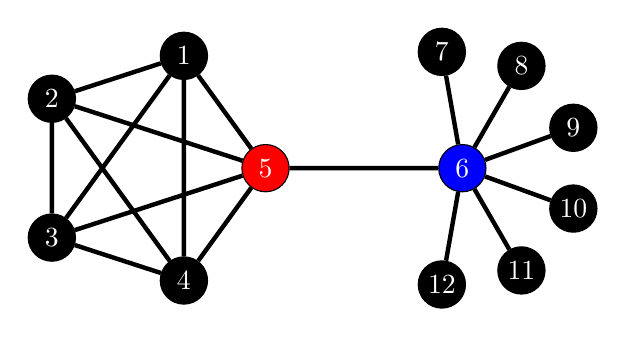
\begin{tikzpicture}[
    main node/.style={circle,fill=black,draw,text=white, minimum size=0.6cm, inner sep=1pt},
    ]
  \def\R{1.5}

  \node[main node] (1) at (72:\R) {1};
  \node[main node] (2) at (144:\R) {2};
  \node[main node] (3) at (216:\R) {3};
  \node[main node] (4) at (288:\R) {4};
  \node[main node, fill=red] (5) at (0:\R) {5};

  \path (5) ++(2.5, 0) node[main node, fill=blue] (6) {6};
  \path (6) ++(100:\R)  node[main node] (7)  {7};
  \path (6) ++(60:\R)  node[main node] (8)  {8};
  \path (6) ++(20:\R)  node[main node] (9)  {9};
  \path (6) ++(-20:\R) node[main node] (10) {10};
  \path (6) ++(-60:\R) node[main node] (11) {11};
  \path (6) ++(-100:\R) node[main node] (12) {12};

  \draw[ultra thick] (5) -- (1) -- (2) -- (3) -- (4) -- (5) -- (2) -- (4) -- (1) -- (3) -- (5) -- (6);
  \draw[ultra thick] (6) -- (7);
  \draw[ultra thick] (6) -- (8);
  \draw[ultra thick] (6) -- (9);
  \draw[ultra thick] (6) -- (10);
  \draw[ultra thick] (6) -- (11);
  \draw[ultra thick] (6) -- (12);
\end{tikzpicture}
\caption{ペアワイズナッシュ均衡でない初期構造のネットワーク例}
\label{fig:3.2}
\end{figure}
図\ref{fig:3.3}のような構造がペアワイズナッシュ均衡となるため, 図\ref{fig:3.2}はペアワイズナッシュ均衡ではない.

\begin{figure}[htbp]
\centering
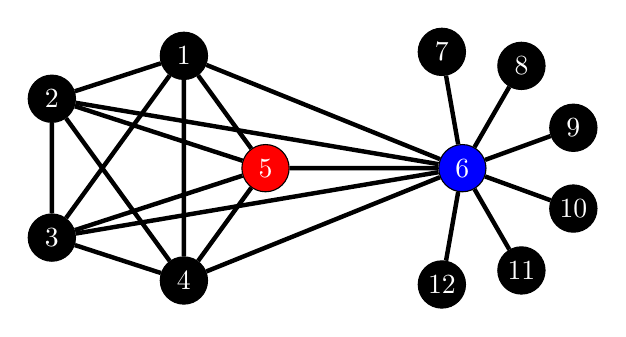
\begin{tikzpicture}[
    main node/.style={circle,fill=black,draw,text=white, minimum size=0.6cm, inner sep=1pt},
    ]
  \def\R{1.5}

  \node[main node] (1) at (72:\R) {1};
  \node[main node] (2) at (144:\R) {2};
  \node[main node] (3) at (216:\R) {3};
  \node[main node] (4) at (288:\R) {4};
  \node[main node, fill=red] (5) at (0:\R) {5};

  \path (5) ++(2.5, 0) node[main node, fill=blue] (6) {6};
  \path (6) ++(100:\R)  node[main node] (7)  {7};
  \path (6) ++(60:\R)  node[main node] (8)  {8};
  \path (6) ++(20:\R)  node[main node] (9)  {9};
  \path (6) ++(-20:\R) node[main node] (10) {10};
  \path (6) ++(-60:\R) node[main node] (11) {11};
  \path (6) ++(-100:\R) node[main node] (12) {12};

  \draw[ultra thick] (5) -- (1) -- (2) -- (3) -- (4) -- (5) -- (2) -- (4) -- (1) -- (3) -- (5) -- (6);
  \draw[ultra thick] (6) -- (7);
  \draw[ultra thick] (6) -- (8);
  \draw[ultra thick] (6) -- (9);
  \draw[ultra thick] (6) -- (10);
  \draw[ultra thick] (6) -- (11);
  \draw[ultra thick] (6) -- (12);

  %ペアワイズナッシュ均衡に収束することで新たに形成されたリンク
  \draw[ultra thick] (6) -- (1);
  \draw[ultra thick] (6) -- (2);
  \draw[ultra thick] (6) -- (3);
  \draw[ultra thick] (6) -- (4);
\end{tikzpicture}
\caption{図\ref{fig:3.2}をペアワイズナッシュ均衡に収束させた場合のネットワーク}
\label{fig:3.3}
\end{figure}
図\ref{fig:3.2}のような初期状態がペアワイズナッシュ均衡にない状況において, intercentralityが最高値となるキープレイヤーのエージェント5を排除した場合よりも, エージェント6を排除した場合の方が総努力水準が低くなることが, シミュレーション結果を示した図\ref{fig:3.6}からわかる.\footnote{それぞれのエージェントのintercentralityは, $c_1(G)=3.8447$, $c_2(G)=3.8447$, $c_3(G)=3.8447$, $c_4(G)=3.8447$, $c_5(G)=4.6171$, $c_6(G)=2.9090$, $c_7(G)=0.6871$, $c_8(G)=0.6871$, $c_9(G)=0.6871$, $c_{10}(G)=0.6871$, $c_{11}(G)=0.6871$, $c_{12}(G)=0.6871$ であるため, エージェント5がキープレイヤーとなる.}
エージェント5を排除したときに割引総努力水準が大きくなっているのは, 初期状態がペアワイズナッシュ均衡になく, $\kappa$ が比較的に小さいため, ネットワークの適応過程において図\ref{fig:3.4}のように新たなリンク形成が発生し, エージェント6が中心的な役割を果たすようになったことが原因である.

\begin{figure}[htbp]
\centering
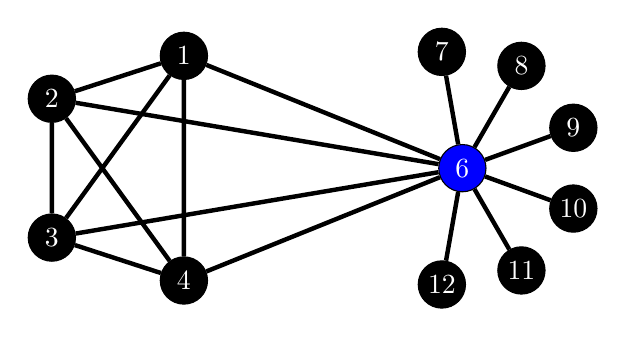
\begin{tikzpicture}[
    main node/.style={circle,fill=black,draw,text=white, minimum size=0.6cm, inner sep=1pt},
    ]
  \def\R{1.5}

  \node[main node] (1) at (72:\R) {1};
  \node[main node] (2) at (144:\R) {2};
  \node[main node] (3) at (216:\R) {3};
  \node[main node] (4) at (288:\R) {4};
  \node[main node, fill=white, draw=none] (5) at (0:\R) {};

  \path (5) ++(2.5, 0) node[main node, fill=blue] (6) {6};
  \path (6) ++(100:\R)  node[main node] (7)  {7};
  \path (6) ++(60:\R)  node[main node] (8)  {8};
  \path (6) ++(20:\R)  node[main node] (9)  {9};
  \path (6) ++(-20:\R) node[main node] (10) {10};
  \path (6) ++(-60:\R) node[main node] (11) {11};
  \path (6) ++(-100:\R) node[main node] (12) {12};

  \draw[ultra thick] (1) -- (2) -- (3) -- (4) -- (1) -- (2) -- (4) -- (1) -- (3);
  \draw[ultra thick] (6) -- (7);
  \draw[ultra thick] (6) -- (8);
  \draw[ultra thick] (6) -- (9);
  \draw[ultra thick] (6) -- (10);
  \draw[ultra thick] (6) -- (11);
  \draw[ultra thick] (6) -- (12);

  %新たに形成されたリンク
  \draw[ultra thick] (6) -- (1);
  \draw[ultra thick] (6) -- (2);
  \draw[ultra thick] (6) -- (3);
  \draw[ultra thick] (6) -- (4);
\end{tikzpicture}
\caption{エージェント5を排除した場合のペアワイズナッシュ均衡ネットワーク}
\label{fig:3.4}
\end{figure}
\begin{figure}[htbp]
\centering
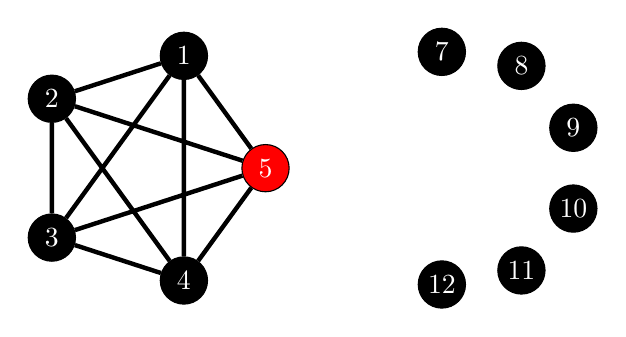
\begin{tikzpicture}[
    main node/.style={circle,fill=black,draw,text=white, minimum size=0.6cm, inner sep=1pt},
    ]
  \def\R{1.5}

  \node[main node] (1) at (72:\R) {1};
  \node[main node] (2) at (144:\R) {2};
  \node[main node] (3) at (216:\R) {3};
  \node[main node] (4) at (288:\R) {4};
  \node[main node, fill=red] (5) at (0:\R) {5};

  \path (5) ++(2.5, 0) node[main node, fill=white, draw=none] (6) {};
  \path (6) ++(100:\R)  node[main node] (7)  {7};
  \path (6) ++(60:\R)  node[main node] (8)  {8};
  \path (6) ++(20:\R)  node[main node] (9)  {9};
  \path (6) ++(-20:\R) node[main node] (10) {10};
  \path (6) ++(-60:\R) node[main node] (11) {11};
  \path (6) ++(-100:\R) node[main node] (12) {12};

  \draw[ultra thick] (5) -- (1) -- (2) -- (3) -- (4) -- (5) -- (2) -- (4) -- (1) -- (3) -- (5);
\end{tikzpicture}
\caption{エージェント6を排除した場合のペアワイズナッシュ均衡ネットワーク}
\label{fig:3.5}
\end{figure}

\begin{figure}[htbp]
    \centering
    \includegraphics[width=0.8\textwidth]{Fig3.6.png}
    \caption{図\ref{fig:3.2}のネットワークにおいて, キープレイヤー(エージェント5)が排除された場合と, エージェント6が排除された場合の割引総努力水準の比較}
    \label{fig:3.6}
\end{figure}
\end{example}
\vspace{0.5cm}

続いて, 一般的な場合 ($e>1$, $\gamma>0$) における命題1の説明を行う. 
パラメータが一般化されたことにより, ネットワークの適応過程が複雑化するため, 一度 $e' \le e$ である $e'$ 人のエージェントを排除するという条件について考える. 
このとき, 排除されるエージェントの数は $e'$ 人で固定されているため, 同じ数のエージェントのネットワークを比較することができるようになり, Ballester et al. (2006) の定理2を適用することが可能になる.

$A \in \mathcal{E}(e)$, $B \in \mathcal{E}(e')$ $(e' \le e)$である2つのエージェント集合において, 各 $t$ 期で, $G_t(A)$ に $e-e'$ 人の孤立したエージェントを追加することで得られる一連の中間ネットワーク (Intermediary Networks) $\tilde{G}_t(A)$ を考える. 
すると, 第0期において $\tilde{G}_0(A) \subset G_0(B)$ が成立するため, 各 $t$ 期においても $\tilde{G}_t(A) \subseteq G_t(B)$ が成立することが示される. 
つまり, 総ナッシュ均衡努力水準は第0期において中間ネットワークで厳密に低く, その後のすべての期間において弱く低い.

次いで, $\tilde{G}_t(A)$ は孤立エージェントの集合 $A \setminus B$ を $G_t(A)$ に追加することで得られることを示す. 
$\gamma$ が十分に小さい場合, 総ナッシュ均衡努力水準は $\tilde{G}_t(A)$ よりも $G_t(A)$ において常に厳密に低く, そのため必然的に $G_t(B)$ よりも厳密に低い. 
結果として, 最適ターゲティング政策は, エージェントの集合 $A \in \mathcal{E}(e)$ を排除することになる.

最後に, もし $G$ が空ネットワークである場合について説明する. 
$\gamma = 0$ の場合は, エージェントの排除後, どの期間においても新しいリンクは形成されない. 
したがって, 最適ターゲティングは $e$ 人のエージェントの任意の集合を排除することとなる. 
他方で, $\gamma > 0$ の場合は, 新しいリンクを形成するための残存エージェントの限界利得は, 排除されるエージェントの数に関して増加する. 
任意の $\gamma > 0$ に対して, $G$ がペアワイズナッシュ均衡ネットワークであり, かつ $G$ からエージェントを排除した後に残存エージェントが新しいリンクを形成することを有益となるようなリンク費用が存在する. 
その場合, $\gamma > 0$ が任意に小さくても介入しないことが最適となる可能性がある. 

\subsection{$\gamma$ が大きい場合の最適ターゲティング}
本節では, グローバルな戦略的代替効果を統御するパラメータ $\gamma$ が大きい場合における最適ターゲティング政策について分析する. 
グローバルな戦略的代替効果が大きい場合, 周辺エージェントを排除することが最適となる可能性がある. 
さらに, 排除可能なすべてのエージェントを排除しないことが最適となる場合があり, そもそも介入することが介入しないことよりも事態を悪化させる可能性もある. 

まず, グローバルな戦略的代替効果が大きい場合, コアエージェント, つまりキープレイヤーをターゲットにすることが最適ではない可能性があることを示す. 
その直感的な解釈は, そのようなエージェントを排除するとグローバルな戦略的代替効果が最も減少し, 残りのエージェントがその後の期間で新しいリンクを形成するようになる可能性があるというものである. 
後の期間におけるより密なネットワークは, 割引因子 $\delta$ が十分に大きい場合, 初期のより疎なネットワークの利点を上回る可能性がある. 
このメカニズムを図示するために, 周辺エージェントを排除することが最適となる以下の例を提示する.

\vspace{0.5cm}
\begin{example}
    $e=1$, $n=8$, $\alpha=1$, $\beta=6$, $\lambda=0.75$, $\gamma=0.74$, $\kappa=0.006$, $\delta=0.99$ を仮定する.
    このとき, 図\ref{fig:3.7}に描かれたネットワーク$G$を仮定し, $G$はペアワイズナッシュ均衡ネットワークである.
    ネットワーク $G$ は, エージェント1からエージェント6は完全ネットワークを形成しているが, エージェント7とエージェント8はそれぞれ孤立している. 
    図\ref{fig:3.7}のとき, ネットワークにおける総努力水準は約0.93である.

    コアエージェント $c$ と, 周辺エージェント $p$ の排除を比較する. 
    このネットワークにおいて, エージェント1からエージェント6がエージェント $c$ であり, エージェント7とエージェント8は周辺エージェント $p$ である.
    コアエージェント$c$であるエージェント4を排除した後のネットワークの適応過程を図\ref{fig:3.8}から図\ref{fig:3.10}に示す. 
    また, 周辺エージェント$p$であるエージェント7を排除した後のネットワークの適応過程を図\ref{fig:3.11}から図\ref{fig:3.13}に示す.

    \begin{figure}[htbp]
        \centering
        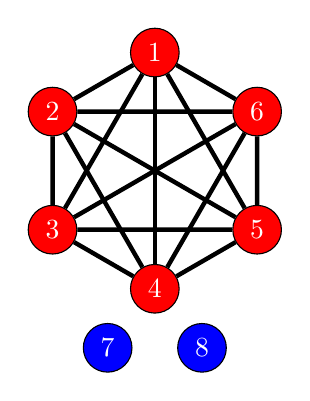
\begin{tikzpicture}[
            main node/.style={circle,fill=black,draw,text=white},
            ]
            \def\R{1.5}
            
            \node[main node, fill=red] (1) at (90:\R) {1};
            \node[main node, fill=red] (2) at (150:\R) {2};
            \node[main node, fill=red] (3) at (210:\R) {3};
            \node[main node, fill=red] (4) at (270:\R) {4};
            \node[main node, fill=red] (5) at (330:\R) {5};
            \node[main node, fill=red] (6) at (30:\R) {6};
            \path (3) ++(0.7, -1.5) node[main node, fill=blue] (7) {7};
            \path (5) ++(-0.7, -1.5) node[main node, fill=blue] (8) {8};
            
            \draw[ultra thick] (1) -- (2) -- (3) -- (4) -- (5) -- (6) -- (1);
            \draw[ultra thick] (1) -- (3) -- (5) -- (1);
            \draw[ultra thick] (2) -- (4) -- (6) -- (2);
            \draw[ultra thick] (1) -- (4);
            \draw[ultra thick] (2) -- (5);
            \draw[ultra thick] (3) -- (6);
        \end{tikzpicture}
        \caption{例7におけるネットワーク$G$}
        \label{fig:3.7}
    \end{figure}

    \begin{figure}[htbp]
    \centering
    \begin{minipage}{0.32\textwidth}
        \centering
        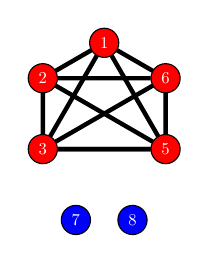
\begin{tikzpicture}[
            scale=0.6, transform shape,
            main node/.style={circle,fill=black,draw,text=white},
            ]
            \def\R{1.5}
            
            \node[main node, fill=red] (1) at (90:\R) {1};
            \node[main node, fill=red] (2) at (150:\R) {2};
            \node[main node, fill=red] (3) at (210:\R) {3};
            \node[main node, fill=red] (5) at (330:\R) {5};
            \node[main node, fill=red] (6) at (30:\R) {6};
            \path (3) ++(0.7, -1.5) node[main node, fill=blue] (7) {7};
            \path (5) ++(-0.7, -1.5) node[main node, fill=blue] (8) {8};
            
            \draw[ultra thick] (1) -- (2) -- (3) -- (5) -- (6) -- (1);
            \draw[ultra thick] (1) -- (3) -- (5) -- (1);
            \draw[ultra thick] (2) -- (6) -- (2) -- (5);
            \draw[ultra thick] (3) -- (6);
        \end{tikzpicture}
        \caption{$G_0(\{c\})$}
        \label{fig:3.8}
    \end{minipage}
    \hfill 
    \begin{minipage}{0.32\textwidth}
        \centering
        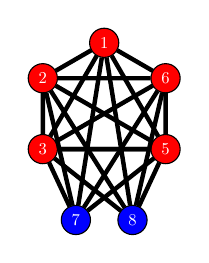
\begin{tikzpicture}[
            scale=0.6, transform shape,
            main node/.style={circle,fill=black,draw,text=white},
            ]
            \def\R{1.5}
            
            \node[main node, fill=red] (1) at (90:\R) {1};
            \node[main node, fill=red] (2) at (150:\R) {2};
            \node[main node, fill=red] (3) at (210:\R) {3};
            \node[main node, fill=red] (5) at (330:\R) {5};
            \node[main node, fill=red] (6) at (30:\R) {6};
            \path (3) ++(0.7, -1.5) node[main node, fill=blue] (7) {7};
            \path (5) ++(-0.7, -1.5) node[main node, fill=blue] (8) {8};
            
            \draw[ultra thick] (1) -- (2) -- (3) -- (5) -- (6) -- (1);
            \draw[ultra thick] (1) -- (3) -- (5) -- (1);
            \draw[ultra thick] (2) -- (6) -- (2) -- (5);
            \draw[ultra thick] (3) -- (6);
            \draw[ultra thick] (7) -- (1);
            \draw[ultra thick] (7) -- (2);
            \draw[ultra thick] (7) -- (3);
            \draw[ultra thick] (7) -- (5);
            \draw[ultra thick] (7) -- (6);
            \draw[ultra thick] (8) -- (1);
            \draw[ultra thick] (8) -- (2);
            \draw[ultra thick] (8) -- (3);
            \draw[ultra thick] (8) -- (5);
            \draw[ultra thick] (8) -- (6);
        \end{tikzpicture}
        \caption{$G_1(\{c\})=G_2(\{c\})$}
        \label{fig:3.9}
    \end{minipage}
    \hfill
    \begin{minipage}{0.32\textwidth}
        \centering
        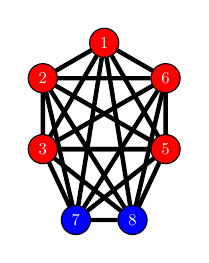
\begin{tikzpicture}[
            scale=0.6, transform shape,
            main node/.style={circle,fill=black,draw,text=white},
            ]
            \def\R{1.5}
            
            \node[main node, fill=red] (1) at (90:\R) {1};
            \node[main node, fill=red] (2) at (150:\R) {2};
            \node[main node, fill=red] (3) at (210:\R) {3};
            \node[main node, fill=red] (5) at (330:\R) {5};
            \node[main node, fill=red] (6) at (30:\R) {6};
            \path (3) ++(0.7, -1.5) node[main node, fill=blue] (7) {7};
            \path (5) ++(-0.7, -1.5) node[main node, fill=blue] (8) {8};
            
            \draw[ultra thick] (1) -- (2) -- (3) -- (5) -- (6) -- (1);
            \draw[ultra thick] (1) -- (3) -- (5) -- (1);
            \draw[ultra thick] (2) -- (6) -- (2) -- (5);
            \draw[ultra thick] (3) -- (6);
            \draw[ultra thick] (7) -- (1);
            \draw[ultra thick] (7) -- (2);
            \draw[ultra thick] (7) -- (3);
            \draw[ultra thick] (7) -- (5);
            \draw[ultra thick] (7) -- (6);
            \draw[ultra thick] (8) -- (1);
            \draw[ultra thick] (8) -- (2);
            \draw[ultra thick] (8) -- (3);
            \draw[ultra thick] (8) -- (5);
            \draw[ultra thick] (8) -- (6);
            \draw[ultra thick] (7) -- (8);
        \end{tikzpicture}
        \caption{$G_t(\{c\}),\ t\geq3$}
        \label{fig:3.10}
    \end{minipage}
\end{figure}

\begin{figure}[htbp]
    \centering
    \begin{minipage}{0.32\textwidth}
        \centering
        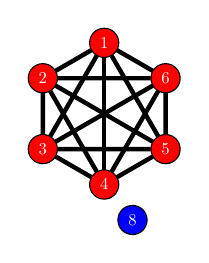
\begin{tikzpicture}[
            scale=0.6, transform shape,
            main node/.style={circle,fill=black,draw,text=white},
            ]
            \def\R{1.5}
            
            \node[main node, fill=red] (1) at (90:\R) {1};
            \node[main node, fill=red] (2) at (150:\R) {2};
            \node[main node, fill=red] (3) at (210:\R) {3};
            \node[main node, fill=red] (4) at (270:\R) {4};
            \node[main node, fill=red] (5) at (330:\R) {5};
            \node[main node, fill=red] (6) at (30:\R) {6};
            \path (5) ++(-0.7, -1.5) node[main node, fill=blue] (8) {8};
            
            \draw[ultra thick] (1) -- (2) -- (3) -- (4) -- (5) -- (6) -- (1);
            \draw[ultra thick] (1) -- (3) -- (5) -- (1);
            \draw[ultra thick] (2) -- (4) -- (6) -- (2);
            \draw[ultra thick] (1) -- (4);
            \draw[ultra thick] (2) -- (5);
            \draw[ultra thick] (3) -- (6);
        \end{tikzpicture}
        \caption{$G_0(\{p\})$}
        \label{fig:3.11}
    \end{minipage}
    \hfill 
    \begin{minipage}{0.32\textwidth}
        \centering
        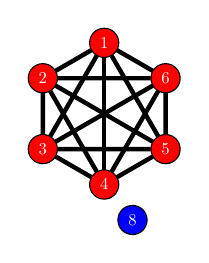
\begin{tikzpicture}[
            scale=0.6, transform shape,
            main node/.style={circle,fill=black,draw,text=white},
            ]
            \def\R{1.5}
            
            \node[main node, fill=red] (1) at (90:\R) {1};
            \node[main node, fill=red] (2) at (150:\R) {2};
            \node[main node, fill=red] (3) at (210:\R) {3};
            \node[main node, fill=red] (4) at (270:\R) {4};
            \node[main node, fill=red] (5) at (330:\R) {5};
            \node[main node, fill=red] (6) at (30:\R) {6};
            \path (5) ++(-0.7, -1.5) node[main node, fill=blue] (8) {8};
            
            \draw[ultra thick] (1) -- (2) -- (3) -- (4) -- (5) -- (6) -- (1);
            \draw[ultra thick] (1) -- (3) -- (5) -- (1);
            \draw[ultra thick] (2) -- (4) -- (6) -- (2);
            \draw[ultra thick] (1) -- (4);
            \draw[ultra thick] (2) -- (5);
            \draw[ultra thick] (3) -- (6);
        \end{tikzpicture}
        \caption{$G_1(\{p\})=G_2(\{p\})$}
        \label{fig:3.12}
    \end{minipage}
    \hfill
    \begin{minipage}{0.32\textwidth}
        \centering
        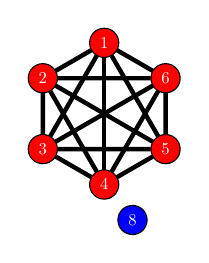
\begin{tikzpicture}[
            scale=0.6, transform shape,
            main node/.style={circle,fill=black,draw,text=white},
            ]
            \def\R{1.5}
            
            \node[main node, fill=red] (1) at (90:\R) {1};
            \node[main node, fill=red] (2) at (150:\R) {2};
            \node[main node, fill=red] (3) at (210:\R) {3};
            \node[main node, fill=red] (4) at (270:\R) {4};
            \node[main node, fill=red] (5) at (330:\R) {5};
            \node[main node, fill=red] (6) at (30:\R) {6};
            \path (5) ++(-0.7, -1.5) node[main node, fill=blue] (8) {8};
            
            \draw[ultra thick] (1) -- (2) -- (3) -- (4) -- (5) -- (6) -- (1);
            \draw[ultra thick] (1) -- (3) -- (5) -- (1);
            \draw[ultra thick] (2) -- (4) -- (6) -- (2);
            \draw[ultra thick] (1) -- (4);
            \draw[ultra thick] (2) -- (5);
            \draw[ultra thick] (3) -- (6);
        \end{tikzpicture}
        \caption{$G_t(\{p\}),\ t\geq3$}
        \label{fig:3.13}
    \end{minipage}
\end{figure}

$G_0(\{p\})$ はペアワイズナッシュ均衡ネットワークであり, すべての $t$ について $G_0(\{p\}) = G_t(\{p\})$ である. 
しかし コアエージェント $c$ を排除すると, ネットワークは適応する. $t=1$ において, 周辺エージェント$p$はコアエージェント$c$とのリンクを形成し, $G_1(\{c\})$ を生じる. 
一方 $t=2$ においては, どのエージェントもリンクの部分集合を削除することで有益に逸脱することはできず, $G_1(\{c\}) = G_2(\{c\})$ となる. 
最後に $t=3$ において, 周辺エージェントは互いにリンクし, $G_t(\{c\})$ は $t \ge 3$ において完全ネットワークとなる. 
    
$G_0(\{c\}) \subset G_0(\{p\})$ である一方で, すべての $t \ge 1$ について $G_t(\{p\}) \subseteq G_t(\{c\})$ が成立することに注意されたい. 
したがって, 総努力水準は $G_0(\{p\})$ よりも $G_0(\{c\})$ において厳密に低く, それぞれ $\sum_{j \in N \setminus \{c\}}x_j \approx 0.81$, $\sum_{j \in N \setminus \{p\}}x_j \approx 0.92$ である. 
しかし, それ以降のすべての期間において $\sum_{j \in N \setminus \{c\}}x_j$ は $\sum_{j \in N \setminus \{p\}}x_j$ より厳密に高く, $t=1$ と $t=2$ では $\sum_{j \in N \setminus \{c\}}x_j \approx 1.02$と$\sum_{j \in N \setminus \{p\}}x_j \approx 0.92$, 任意の $t \ge 3$ では $\sum_{j \in N \setminus \{c\}}x_j \approx 1.05$ と $\sum_{j \in N \setminus \{p\}}x_j \approx 0.92$ である. 
$\delta=0.99$ の場合, 割引総努力水準は, 介入しないときに約93.17, $p$を排除した場合に約91.50, $c$を排除した場合に約100.45となる. 
したがって, 周辺エージェント $p$ を排除することが例7においては最適である.
\end{example}
\vspace{0.5cm}

例8では, 最大数 $e$ のエージェントを排除することが最適ではない場合があることを示す. 
その直感解釈は以下の通りである. 
すべての $e$ 人のエージェントを排除すると, 当初はより少ないエージェントの疎なネットワークになる. 
しかし, グローバルな戦略的代替効果のより大きな減少により, 残りのエージェントは後の期間においてより多くのリンクを形成する可能性がある. 
より少ないエージェントによる密なネットワークは, 割引因子 $\delta$ が十分に大きい場合, より多くのエージェントによる疎なネットワークの利点を上回る可能性がある\footnote{ターゲティング費用(排除に必要な費用)がなくても, より少ないエージェントを排除することが最適となる場合があることに注意されたい. 排除されるエージェントの数において単調増加するターゲティング費用関数を仮定した場合にも, 同様の結果を得ることができる.}. 
同じ理由で, 介入しないことが介入することよりも良い結果をもたらす可能性がある. 
これらの結果は, 戦略的代替効果が十分に小さい場合には生じないことに注意されたい. 
その場合, エージェントは新しいリンクを決して形成せず, 既存のリンクを削除する最も強いインセンティブを持つ. 
その結果, 最も次数の高い $e$ 人のエージェントすべてを排除することで, すべての期間において最も少ないエージェントによる最も疎なネットワークが得られ, したがってこのターゲティング政策が最適となる.

\vspace{0.5cm}
\begin{example}
    $e=2$, $n=8$, $\alpha=4.5$, $\beta=7.375$, $\lambda=1$, $\gamma=0.75$, $\kappa=0.15625$, $\delta$が十分に大きい場合を仮定する. 
    このとき, 図\ref{fig:3.14}に描かれたネットワーク$G$を仮定し, $G$はペアワイズナッシュ均衡ネットワークである. 
    ネットワーク $G$ は, エージェント1を中心とするスター型ネットワークである. 
    このときの総努力水準は約3.2である. 
    このネットワークにおいては, エージェント1がコアエージェント $c$ であり, エージェント2からエージェント8が周辺エージェント $p$ である.
    ここでは, コアエージェント$c$であるエージェント1のみを排除した場合と, エージェント1と周辺エージェント$p$であるエージェント2の両方を排除した場合を比較する. 

    エージェント1のみを排除した後のネットワークの適応過程を図\ref{fig:3.15}と図\ref{fig:3.16}に示す. 
    また, エージェント1とエージェント2の両方を排除した後のネットワークの適応過程を図\ref{fig:3.17}と図\ref{fig:3.18}に示す.

    \begin{figure}[htbp]
        \centering
        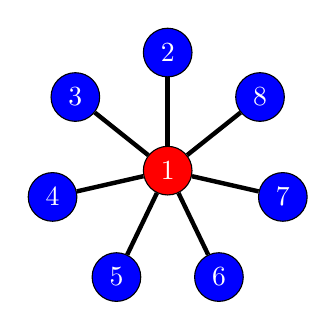
\begin{tikzpicture}[
            main node/.style={circle,fill=black,draw,text=white},
            ]
            
            \node[main node, fill=red] (1) at (0,0) {1};
            
            \node[main node, fill=blue] (2) at (90:1.5cm) {2};
            \node[main node, fill=blue] (3) at ({90 + 360/7}:1.5cm) {3};
            \node[main node, fill=blue] (4) at ({90 + 360/7 * 2}:1.5cm) {4};
            \node[main node, fill=blue] (5) at ({90 + 360/7 * 3}:1.5cm) {5};
            \node[main node, fill=blue] (6) at ({90 + 360/7 * 4}:1.5cm) {6};
            \node[main node, fill=blue] (7) at ({90 + 360/7 * 5}:1.5cm) {7};
            \node[main node, fill=blue] (8) at ({90 + 360/7 * 6}:1.5cm) {8};
            
            \draw[ultra thick] (1) -- (2);
            \draw[ultra thick] (1) -- (3);
            \draw[ultra thick] (1) -- (4);
            \draw[ultra thick] (1) -- (5);
            \draw[ultra thick] (1) -- (6);
            \draw[ultra thick] (1) -- (7);
            \draw[ultra thick] (1) -- (8);
        \end{tikzpicture}
        \caption{例8におけるネットワーク$G$}
        \label{fig:3.14}
    \end{figure}

    \begin{figure}[htbp]
    \centering
    \begin{minipage}{0.48\textwidth}
        \centering
        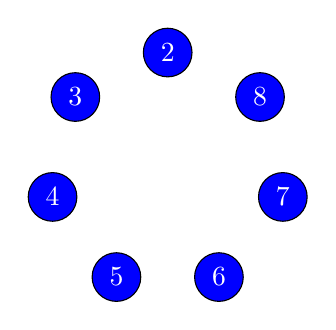
\begin{tikzpicture}[
            main node/.style={circle,fill=black,draw,text=white},
            ]
            
            \node[main node, fill=blue] (2) at (90:1.5cm) {2};
            \node[main node, fill=blue] (3) at ({90 + 360/7}:1.5cm) {3};
            \node[main node, fill=blue] (4) at ({90 + 360/7 * 2}:1.5cm) {4};
            \node[main node, fill=blue] (5) at ({90 + 360/7 * 3}:1.5cm) {5};
            \node[main node, fill=blue] (6) at ({90 + 360/7 * 4}:1.5cm) {6};
            \node[main node, fill=blue] (7) at ({90 + 360/7 * 5}:1.5cm) {7};
            \node[main node, fill=blue] (8) at ({90 + 360/7 * 6}:1.5cm) {8};
        \end{tikzpicture}
        \caption{$G_0(\{c\})$}
        \label{fig:3.15}
    \end{minipage}
    \hfill 
    \begin{minipage}{0.48\textwidth}
        \centering
        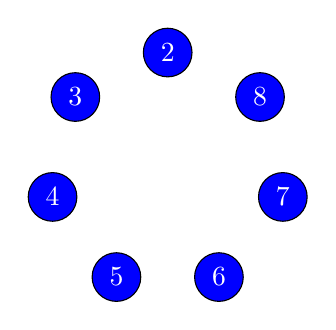
\begin{tikzpicture}[
            main node/.style={circle,fill=black,draw,text=white},
            ]
            
            \node[main node, fill=blue] (2) at (90:1.5cm) {2};
            \node[main node, fill=blue] (3) at ({90 + 360/7}:1.5cm) {3};
            \node[main node, fill=blue] (4) at ({90 + 360/7 * 2}:1.5cm) {4};
            \node[main node, fill=blue] (5) at ({90 + 360/7 * 3}:1.5cm) {5};
            \node[main node, fill=blue] (6) at ({90 + 360/7 * 4}:1.5cm) {6};
            \node[main node, fill=blue] (7) at ({90 + 360/7 * 5}:1.5cm) {7};
            \node[main node, fill=blue] (8) at ({90 + 360/7 * 6}:1.5cm) {8};
        \end{tikzpicture}
        \caption{$G_t(\{c\}),\ t\geq1$}
        \label{fig:3.16}
    \end{minipage}
    \hfill
\end{figure}

    \begin{figure}[htbp]
    \centering
    \begin{minipage}{0.48\textwidth}
        \centering
        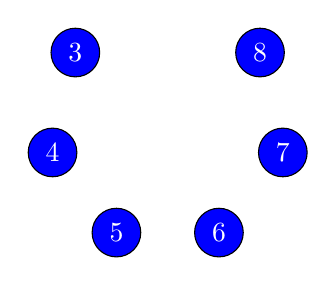
\begin{tikzpicture}[
            main node/.style={circle,fill=black,draw,text=white},
            ]
            
            \node[main node, fill=blue] (3) at ({90 + 360/7}:1.5cm) {3};
            \node[main node, fill=blue] (4) at ({90 + 360/7 * 2}:1.5cm) {4};
            \node[main node, fill=blue] (5) at ({90 + 360/7 * 3}:1.5cm) {5};
            \node[main node, fill=blue] (6) at ({90 + 360/7 * 4}:1.5cm) {6};
            \node[main node, fill=blue] (7) at ({90 + 360/7 * 5}:1.5cm) {7};
            \node[main node, fill=blue] (8) at ({90 + 360/7 * 6}:1.5cm) {8};
        \end{tikzpicture}
        \caption{$G_0(\{c, p\})$}
        \label{fig:3.17}
    \end{minipage}
    \hfill 
    \begin{minipage}{0.48\textwidth}
        \centering
        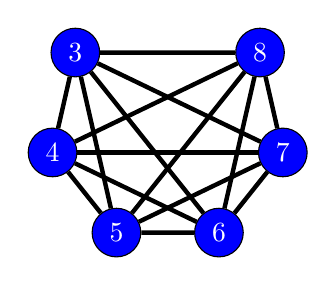
\begin{tikzpicture}[
            main node/.style={circle,fill=black,draw,text=white},
            ]

            \node[main node, fill=blue] (3) at ({90 + 360/7}:1.5cm) {3};
            \node[main node, fill=blue] (4) at ({90 + 360/7 * 2}:1.5cm) {4};
            \node[main node, fill=blue] (5) at ({90 + 360/7 * 3}:1.5cm) {5};
            \node[main node, fill=blue] (6) at ({90 + 360/7 * 4}:1.5cm) {6};
            \node[main node, fill=blue] (7) at ({90 + 360/7 * 5}:1.5cm) {7};
            \node[main node, fill=blue] (8) at ({90 + 360/7 * 6}:1.5cm) {8};
            
            \draw[ultra thick] (3) -- (4) -- (5) -- (6) -- (7) -- (8) -- (3);
            \draw[ultra thick] (3) -- (5) -- (7) -- (3);
            \draw[ultra thick] (4) -- (6) -- (8) -- (4);
            \draw[ultra thick] (3) -- (6);
            \draw[ultra thick] (4) -- (7);
            \draw[ultra thick] (5) -- (8);
        \end{tikzpicture}
        \caption{$G_t(\{c, p\}),\ t\geq1$}
        \label{fig:3.18}
    \end{minipage}
    \hfill
\end{figure}

コアエージェント$c$のみを排除すると, すべての期間において $n-1$ 人のエージェントの空ネットワークが得られ, 総努力水準は約2.5となる. 
コアエージェント$c$と周辺エージェント$p$を排除すると, 第0期において $n-2$ 人のエージェントの空ネットワークが得られ, 総努力水準は約2.3となる. 
第1期以降, ネットワークは $n-2$ 人のエージェントの完全ネットワークとなり, 総努力水準は約3.9となる. 
すなわち, $\delta$ が十分に大きい場合, コアエージェント$c$のみを排除することが最適である. 
コアエージェント$c$と周辺エージェント$p$の両方を排除することは, ネットワークが適応する場合においては, 介入しないよりも悪い結果を招くことが確認された.
\end{example}
\vspace{0.5cm}

以上, グローバルな戦略的代替効果が大きい場合において, 固定ネットワークを前提とした直感とは異なる逆説的な結果が得られることを示した. 
上記に示した例はすべて, 初期ネットワークがペアワイズナッシュ均衡ネットワークである場合であった. 
次に, 初期ネットワークがペアワイズナッシュ均衡ネットワークでない場合においても, 同様の逆説的な結果が得られることを示す.

\vspace{0.5cm}
\begin{example}
    $e=2$, $n=11$, $\alpha=1.0$, $\beta=8.0$, $\lambda=1.0$, $\gamma=0.60$, $\kappa=0.01$, $\delta=0.95$を仮定する. 
    このとき, 図\ref{fig:3.19}に描かれたネットワーク$G$を仮定する.
    このとき, エージェント5がコアエージェント $c$ であり, それ以外が周辺エージェント $p$ である. 特に本例では, 最もintercentralityが小さいエージェント7に着目する.

    どのエージェントも排除せずに放置した後のネットワークが安定した状態を図\ref{fig:3.20}に示す. 
    コアエージェント$c$(エージェント5)のみを排除した後のネットワークが安定した状態を図\ref{fig:3.21}に示し, 周辺エージェント$p$(エージェント7)のみを排除した後のネットワークが安定した状態を図\ref{fig:3.22}に示す. 
    また, コアエージェント$c$と周辺エージェント$p$の両方(エージェント5とエージェント7)を排除した後のネットワークが安定した状態を図\ref{fig:3.23}に示す.
    そして, 以上のすべての$t$期における努力水準の推移や, 割引総努力水準を書いたグラフを図\ref{fig:3.24}として提示する.

    \begin{figure}[htbp]
        \centering
        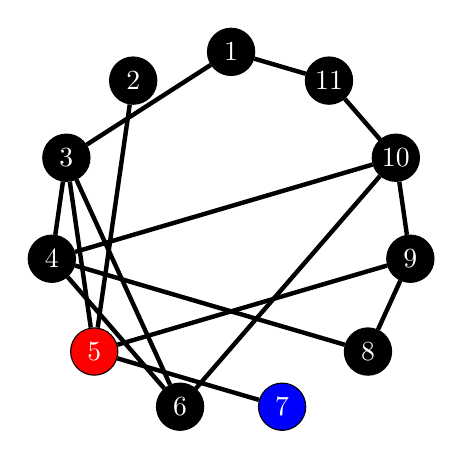
\begin{tikzpicture}[
            main node/.style={circle,fill=black,draw,text=white, minimum size=0.6cm, inner sep=1pt},
            ]
            \def\R{2.3}
            
            \node[main node] (1) at (90:\R) {1};
            \node[main node] (2) at (90+360/11*1:\R) {2};
            \node[main node] (3) at (90+360/11*2:\R) {3};
            \node[main node] (4) at (90+360/11*3:\R) {4};
            \node[main node, fill=red] (5) at (90+360/11*4:\R) {5};
            \node[main node] (6) at (90+360/11*5:\R) {6};
            \node[main node, fill=blue] (7) at (90+360/11*6:\R) {7};
            \node[main node] (8) at (90+360/11*7:\R) {8};
            \node[main node] (9) at (90+360/11*8:\R) {9};
            \node[main node] (10) at (90+360/11*9:\R) {10};
            \node[main node] (11) at (90+360/11*10:\R) {11};

            \draw[ultra thick] (1) -- (3);
            \draw[ultra thick] (1) -- (11);
            \draw[ultra thick] (2) -- (5);
            \draw[ultra thick] (3) -- (4);
            \draw[ultra thick] (3) -- (5);
            \draw[ultra thick] (3) -- (6);
            \draw[ultra thick] (4) -- (6);
            \draw[ultra thick] (4) -- (8);
            \draw[ultra thick] (4) -- (10);
            \draw[ultra thick] (5) -- (7);
            \draw[ultra thick] (5) -- (9);
            \draw[ultra thick] (6) -- (10);
            \draw[ultra thick] (8) -- (9);
            \draw[ultra thick] (9) -- (10);
            \draw[ultra thick] (10) -- (11);
        \end{tikzpicture}
        \caption{例9におけるネットワーク$G$}
        \label{fig:3.19}
    \end{figure}

    \begin{figure}[htbp]
    \centering
    \begin{minipage}{0.48\textwidth}
        \centering
        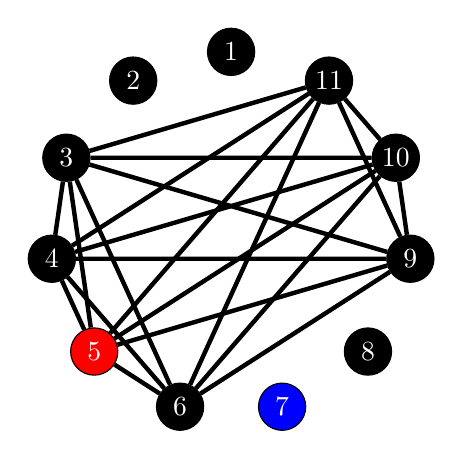
\begin{tikzpicture}[
            main node/.style={circle,fill=black,draw,text=white, minimum size=0.6cm, inner sep=1pt},
            ]
            \def\R{2.3}
            
            \node[main node] (1) at (90:\R) {1};
            \node[main node] (2) at (90+360/11*1:\R) {2};
            \node[main node] (3) at (90+360/11*2:\R) {3};
            \node[main node] (4) at (90+360/11*3:\R) {4};
            \node[main node, fill=red] (5) at (90+360/11*4:\R) {5};
            \node[main node] (6) at (90+360/11*5:\R) {6};
            \node[main node, fill=blue] (7) at (90+360/11*6:\R) {7};
            \node[main node] (8) at (90+360/11*7:\R) {8};
            \node[main node] (9) at (90+360/11*8:\R) {9};
            \node[main node] (10) at (90+360/11*9:\R) {10};
            \node[main node] (11) at (90+360/11*10:\R) {11};

            \draw[ultra thick] (3) -- (4) -- (5) -- (6) -- (9) -- (10) -- (11) -- (3);
            \draw[ultra thick] (3) -- (5);
            \draw[ultra thick] (3) -- (6);
            \draw[ultra thick] (3) -- (9);
            \draw[ultra thick] (3) -- (10);
            \draw[ultra thick] (4) -- (6);
            \draw[ultra thick] (4) -- (9);
            \draw[ultra thick] (4) -- (10);
            \draw[ultra thick] (4) -- (11);
            \draw[ultra thick] (5) -- (9);
            \draw[ultra thick] (5) -- (10);
            \draw[ultra thick] (5) -- (11);
            \draw[ultra thick] (6) -- (10);
            \draw[ultra thick] (6) -- (11);
            \draw[ultra thick] (9) -- (11);
        \end{tikzpicture}
        \caption{$G_t,\ t\geq3$}
        \label{fig:3.20}
    \end{minipage}
    \hfill 
    \begin{minipage}{0.48\textwidth}
        \centering
        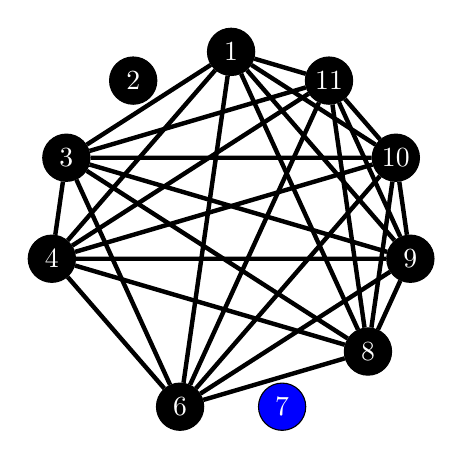
\begin{tikzpicture}[
            main node/.style={circle,fill=black,draw,text=white, minimum size=0.6cm, inner sep=1pt},
            ]
            \def\R{2.3}
            
            \node[main node] (1) at (90:\R) {1};
            \node[main node] (2) at (90+360/11*1:\R) {2};
            \node[main node] (3) at (90+360/11*2:\R) {3};
            \node[main node] (4) at (90+360/11*3:\R) {4};
            \node[main node] (6) at (90+360/11*5:\R) {6};
            \node[main node, fill=blue] (7) at (90+360/11*6:\R) {7};
            \node[main node] (8) at (90+360/11*7:\R) {8};
            \node[main node] (9) at (90+360/11*8:\R) {9};
            \node[main node] (10) at (90+360/11*9:\R) {10};
            \node[main node] (11) at (90+360/11*10:\R) {11};

            \draw[ultra thick] (1) -- (3) -- (4) -- (6) -- (8) -- (9) -- (10) -- (11) -- (1);
            \draw[ultra thick] (1) -- (4);
            \draw[ultra thick] (1) -- (6);
            \draw[ultra thick] (1) -- (8);
            \draw[ultra thick] (1) -- (9);
            \draw[ultra thick] (1) -- (10);
            \draw[ultra thick] (3) -- (6);
            \draw[ultra thick] (3) -- (8);
            \draw[ultra thick] (3) -- (9);
            \draw[ultra thick] (3) -- (10);
            \draw[ultra thick] (3) -- (11);
            \draw[ultra thick] (4) -- (8);
            \draw[ultra thick] (4) -- (9);
            \draw[ultra thick] (4) -- (10);
            \draw[ultra thick] (4) -- (11);
            \draw[ultra thick] (6) -- (9);
            \draw[ultra thick] (6) -- (10);
            \draw[ultra thick] (6) -- (11);
            \draw[ultra thick] (8) -- (10);
            \draw[ultra thick] (8) -- (11);
            \draw[ultra thick] (9) -- (11);
        \end{tikzpicture}
        \caption{$G_t(\{c\}),\ t\geq5$}
        \label{fig:3.21}
    \end{minipage}
    \hfill
\end{figure}

    \begin{figure}[htbp]
    \centering
    \begin{minipage}{0.48\textwidth}
        \centering
        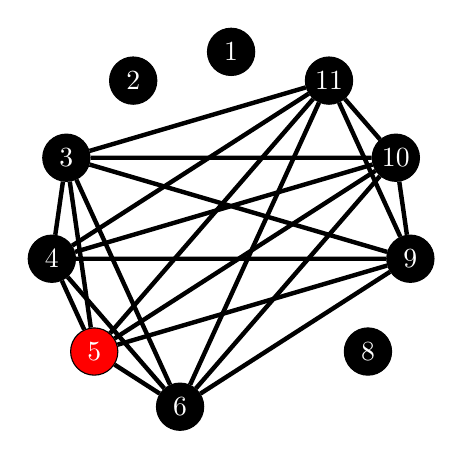
\begin{tikzpicture}[
            main node/.style={circle,fill=black,draw,text=white, minimum size=0.6cm, inner sep=1pt},
            ]
            \def\R{2.3}

            \node[main node] (1) at (90:\R) {1};
            \node[main node] (2) at (90+360/11*1:\R) {2};
            \node[main node] (3) at (90+360/11*2:\R) {3};
            \node[main node] (4) at (90+360/11*3:\R) {4};
            \node[main node, fill=red] (5) at (90+360/11*4:\R) {5};
            \node[main node] (6) at (90+360/11*5:\R) {6};
            \node[main node] (8) at (90+360/11*7:\R) {8};
            \node[main node] (9) at (90+360/11*8:\R) {9};
            \node[main node] (10) at (90+360/11*9:\R) {10};
            \node[main node] (11) at (90+360/11*10:\R) {11};

            \draw[ultra thick] (3) -- (4) -- (5) -- (6) -- (9) -- (10) -- (11) -- (3);
            \draw[ultra thick] (3) -- (5);
            \draw[ultra thick] (3) -- (6);
            \draw[ultra thick] (3) -- (9);
            \draw[ultra thick] (3) -- (10);
            \draw[ultra thick] (4) -- (6);
            \draw[ultra thick] (4) -- (9);
            \draw[ultra thick] (4) -- (10);
            \draw[ultra thick] (4) -- (11);
            \draw[ultra thick] (5) -- (9);
            \draw[ultra thick] (5) -- (10);
            \draw[ultra thick] (5) -- (11);
            \draw[ultra thick] (6) -- (10);
            \draw[ultra thick] (6) -- (11);
            \draw[ultra thick] (9) -- (11);
        \end{tikzpicture}
        \caption{$G_t(\{p\}),\ t\geq3$}
        \label{fig:3.22}
    \end{minipage}
    \hfill 
    \begin{minipage}{0.48\textwidth}
        \centering
        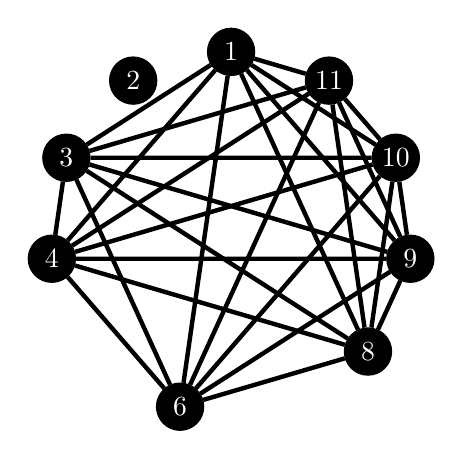
\begin{tikzpicture}[
            main node/.style={circle,fill=black,draw,text=white, minimum size=0.6cm, inner sep=1pt},
            ]
            \def\R{2.3}
            
            \node[main node] (1) at (90:\R) {1};
            \node[main node] (2) at (90+360/11*1:\R) {2};
            \node[main node] (3) at (90+360/11*2:\R) {3};
            \node[main node] (4) at (90+360/11*3:\R) {4};
            \node[main node] (6) at (90+360/11*5:\R) {6};
            \node[main node] (8) at (90+360/11*7:\R) {8};
            \node[main node] (9) at (90+360/11*8:\R) {9};
            \node[main node] (10) at (90+360/11*9:\R) {10};
            \node[main node] (11) at (90+360/11*10:\R) {11};

            \draw[ultra thick] (1) -- (3) -- (4) -- (6) -- (8) -- (9) -- (10) -- (11) -- (1);
            \draw[ultra thick] (1) -- (4);
            \draw[ultra thick] (1) -- (6);
            \draw[ultra thick] (1) -- (8);
            \draw[ultra thick] (1) -- (9);
            \draw[ultra thick] (1) -- (10);
            \draw[ultra thick] (3) -- (6);
            \draw[ultra thick] (3) -- (8);
            \draw[ultra thick] (3) -- (9);
            \draw[ultra thick] (3) -- (10);
            \draw[ultra thick] (3) -- (11);
            \draw[ultra thick] (4) -- (8);
            \draw[ultra thick] (4) -- (9);
            \draw[ultra thick] (4) -- (10);
            \draw[ultra thick] (4) -- (11);
            \draw[ultra thick] (6) -- (9);
            \draw[ultra thick] (6) -- (10);
            \draw[ultra thick] (6) -- (11);
            \draw[ultra thick] (8) -- (10);
            \draw[ultra thick] (8) -- (11);
            \draw[ultra thick] (9) -- (11);
        \end{tikzpicture}
        \caption{$G_t(\{c, p\}),\ t\geq3$}
        \label{fig:3.23}
    \end{minipage}
    \hfill
\end{figure}

\begin{figure}[htbp]
    \centering
    \includegraphics[width=0.8\textwidth]{fig3.24.png}
    \caption{例9におけるターゲティング政策の比較}
    \label{fig:3.24}
\end{figure}
    例9における割引総努力水準を比較すると, 誰も排除しなかった場合は約23.21, コアエージェント$c$のみを排除した場合は約26.41, 周辺エージェント$p$のみを排除した場合は約23.06, コアエージェント$c$と周辺エージェント$p$の両方を排除した場合は約26.71となる.
    つまり, 例9においては, コアエージェント$c$を排除することが必ずしも最適ターゲティングになるとは限らず, また, より多くのエージェントを排除しても必ずしも良い結果になるとはいえない.
\end{example}
\vspace{0.5cm}

このことから, 戦略的代替効果が大きい場合には, 初期状態がペアワイズナッシュ均衡にないネットワークにおいても, 逆説的な結果が得られることが示された. 

したがって, 戦略的代替性の大きさによらず, ペアワイズナッシュ均衡に落ち着いていないネットワークに関しては, intercentralityによるターゲティングは最適ターゲティングにはならず, むしろ事態を悪化させる可能性もあることが明らかとなった.

\section{結論と展望}
本論文は, エージェントが他者の排除後に努力水準およびリンク形成の意思決定を調整する適応的ネットワークにおける最適ターゲティング政策を分析し, ネットワークの適応性とグローバルな戦略代替効果が政策決定に与える重要性を明らかにした. 

分析の結果, グローバルな戦略的代替性が十分に小さく, 初期状態がペアワイズナッシュ均衡にある場合には, 最適ターゲティング政策は最もintercentralityが大きい人物を排除するという単純なルールに帰着し, これはネットワークが固定されている場合の既存の知見と整合的であることが示された. 

一方で, グローバルな戦略的代替効果が大きい場合には, 固定ネットワークの直感とは異なる逆説的な結果が得られた. 
具体的には, intercentralityの低いエージェントを排除することや, 排除可能な最大人数枠を使い切らずに介入を手控えることが最適となる可能性があることが示せた. 

また, ペアワイズナッシュ均衡にないネットワークに介入する場合, 戦略的代替性の大きさにかかわらず, 固定ネットワークの直感とは異なる結果となる可能性が明らかとなった.

結論として, ネットワークが適応的である場合に固定ネットワークを前提とした政策を適用することは, 新規リンクの形成によるリバウンドを招き, 介入を行わない場合よりも事態を悪化させるリスクがあることが示唆された. 

本論文の分析枠組みは, ネットワーク経済学における政策介入の動学的側面を捉える上で有用であるが, 現実社会の複雑な課題に適用するためには, さらなる理論の深堀りと拡張が必要である. 
今後の展望として, 以下の4点が挙げられる. 

第一に, 救済政策 (Rescue Policy) への応用である. 
本論文では犯罪組織の摘発などを念頭に, ネットワーク機能の毀損を目的とした排除に焦点を当てた. 
しかし, 金融ネットワークにおける危機波及の防止や, 共同研究開発 (R\&D) ネットワークにおけるイノベーション促進など, 政策目的がネットワーク機能の維持・向上にある場合も多い. 
特定の重要なエージェントに対して資本注入や補助金といった正のショックを与えることで, 社会厚生を最大化するような最適な救済対象の選定問題へ本モデルを応用することは, 喫緊の課題である. 

第二に, 情報の不完備性の導入である. 
本分析では, 計画者がネットワーク構造の全貌を把握している完全情報を仮定した. 
しかし, テロリスト・ネットワークや地下経済においては, リンクの存在自体が隠蔽されている場合が多く, 観測データにはノイズが含まれる. 
ネットワーク構造に関する情報が不完全である場合や, エージェントのタイプに不確実性が存在する場合において, 誤った推計に基づく介入が適応過程を通じてどのような意図せぬ副作用をもたらすかを検証し, 頑健な政策を構築する必要がある. 

第三に, ターゲティング費用の異質性の考慮である. 
本モデルでは, 排除可能なエージェントの上限数 $e$ を一律の制約条件とした. 
しかし現実には, ネットワークの中心に位置するハブ的な主体ほど防御が堅固であり, その排除には周辺的な主体よりも多大な費用\footnote{費用として, 探索費用, 法的費用, 政治的費用などが考えられる.}を要すると考えられる. 
エージェントの中心性指標に依存したターゲティング費用関数を導入し, 予算制約下での費用対効果を明示的に扱うことで, より現実的な政策提言が可能となるだろう. 

第四に, グラフ理論などに基づいた理論的分析の深化である.
本論文では主に数値シミュレーションを通じて, 戦略的代替性が大きい場合に周辺主体への介入が最適となるケースを示した. 
今後はこのメカニズムについて, より厳密な数学的解析が求められる. 
具体的には, どのようなネットワーク構造において努力水準のリバウンドが支配的となるのか, その境界条件や構造的性質を解析的に特定することは, 政策の予見可能性を高める上で極めて重要な課題である.

これらの拡張は, 適応的ネットワークにおける政策介入の理解を深め, より効果的かつ安全な制度設計に寄与するものである.

\section*{謝辞}
本論文を進めるにあたり, 多大なるご指導, ご鞭撻を賜りました, 指導教員である筑波大学社会・国際学群社会学類の福住多一准教授に, 深く感謝の意を表します. 
福住先生には, 研究テーマの選定から論文の執筆に至るまで, 終始熱心なご指導をいただきました. 
また, 本論文の遂行にあたり, 先生からは多くの有益な助言と温かい励ましをいただきました.
先生の広い見識と研究に対する真摯な姿勢は, 私にとって大きな目標となりました. 

日々の議論を通じて多くの刺激を共有した福住ゼミの皆様にも深く感謝いたします. おかげで, 充実した研究生活を送ることができました. ありがとうございました.

最後に, 長い学生生活を経済的, 精神的に支え続け, 私の進路を温かく見守ってくれた両親には, 感謝の念にたえません. 本当にありがとうございました.

\begin{thebibliography}{9}

\bibitem{BCZ2006}
Ballester, C., Calv\'{o}-Armengol, A. and Zenou, Y. (2006).
``Who's Who in Networks. Wanted: The Key Player,''
\textit{Econometrica}, 74(5), 1403--1417.

\bibitem{BCZ2010}
Ballester, C., Calv\'{o}-Armengol, A. and Zenou, Y. (2010).
``Delinquent Networks,''
\textit{Journal of the European Economic Association}, 8(1), 34--61.

\bibitem{Jackson2008}
Jackson, M. O. (2008).
\textit{Social and Economic Networks}, Princeton University Press.

\bibitem{Hiller2025}
Hiller, T. (2025).
``Targeting in Adaptive Networks,''
\textit{Journal of Economic Theory}, 228, 106059.
\end{thebibliography}
\end{document}

